           \documentclass[twoside]{article}

\usepackage{aistats2023}
% If your paper is accepted, change the options for the package
% aistats2023 as follows:
%
%\usepackage[accepted]{aistats2023}
%
% This option will print headings for the title of your paper and
% headings for the authors names, plus a copyright note at the end of
% the first column of the first page.

% If you set papersize explicitly, activate the following three lines:
%\special{papersize = 8.5in, 11in}
%\setlength{\pdfpageheight}{11in}
%\setlength{\pdfpagewidth}{8.5in}

% If you use natbib package, activate the following three lines:
\usepackage[round]{natbib}
\renewcommand{\bibname}{References}
\renewcommand{\bibsection}{\subsubsection*{\bibname}}
\bibliographystyle{plainnat}
\usepackage{amsmath}
\usepackage{amssymb}
\DeclareMathOperator*{\argmin}{arg\,min}
\usepackage{amsthm}
\newtheorem{theorem}{Theorem}[section]
\newtheorem{corollary}{Corollary}[theorem]
\newtheorem{lemma}[theorem]{Lemma}

\usepackage{xfrac}
\usepackage{hyperref}
\usepackage{graphicx}
\graphicspath{ {./../examples/} }
% If you use BibTeX in apalike style, activate the following line:
%\bibliographystyle{apalike}

\usepackage{tikz}
\usetikzlibrary{matrix,positioning,arrows.meta,arrows,fit,backgrounds,decorations.pathreplacing}
\tikzset{ mymat/.style={ matrix of math nodes, text height=2.5ex, text
depth=0.75ex, text width=6.00ex, align=center, column
sep=-\pgflinewidth, nodes={minimum height=5.0ex} }, mymats/.style={
mymat, nodes={draw,fill=#1} }, mymat2/.style={ matrix of math nodes,
text height=1.0ex, text depth=0.0ex, minimum width=5ex, % text
width=7.00ex, align=center, column sep=-\pgflinewidth }, }
\usetikzlibrary{shapes.geometric, arrows, backgrounds, scopes}
\usepackage{pgfplots} \pgfplotsset{width=6.75cm, compat=newest}
\usepackage[utf8]{inputenc} \DeclareUnicodeCharacter{2212}{−}
\usepgfplotslibrary{groupplots,dateplot}
\usetikzlibrary{patterns,shapes.arrows}



\newcommand{\dfdx}{f^s}
\newcommand{\xc}{\mathbf{x}_c}
\newcommand{\DY}{\mathbf{\Delta Y}}
\newcommand{\xb}{\mathbf{x}}
\newcommand{\Xcb}{\mathbf{X}_c}
\newcommand{\Xb}{\mathcal{X}}
\newcommand{\todo}[1]{[\textcolor{red}{#1}]}

\begin{document}

\twocolumn[

\aistatstitle{Uncertainty-aware Accumulated Local Effects (UALE) for quantifying the heterogeneity of instance-level feature effects}

\aistatsauthor{ Author 1 \And Author 2 \And  Author 3 }

\aistatsaddress{ Institution 1 \And  Institution 2 \And Institution 3 } ]

\begin{abstract}
Accumulated Local Effects (ALE) is a popular explainable AI method that quantifies how a feature influences the decisions of a model, handling well feature correlations. In case of complex interactions between features, instance-level feature effects may deviate from the ALE curve. It is therefore crucial to quantify this deviation, namely, the uncertainty of the effect. In this work, we define Uncertainty-aware ALE (UALE) to quantify and visualize, on a single plot, both the average effect and its uncertainty. We show that UALE quantifies uncertainty effectively, even in case of correlated features. We also note that as in ALE, UALE's approximation requires partitioning the feature domain into non-overlapping intervals (bin-splitting). The average effect and the uncertainty are computed from the instances that lie in each bin. We formally prove that to achieve an unbiased approximation of the uncertainty in each bin, bin-splitting must follow specific constraints. Based on this, we propose a method to determine the optimal intervals, \todo{balancing the estimation bias and variance.} We demonstrate, through synthetic and real datasets, (a) the advantages of modeling the uncertainty with UALE compared to alternative methods and (b) the effectiveness of UALE's appropriate bin splitting for a \todo{good} approximating of the average effect and its uncertainty.
\end{abstract}


\section{INTRODUCTION}

Recently, Machine Learning (ML) has been widely adopted in mission critical domains,
such as healthcare and finance. In such high-stakes areas,  it is important not only to provide accurate predictions but also meaningful explanations. For this reason, there is an increased interest in Explainable
AI (XAI). XAI literature distinguishes between local and global
methods~\citep{Molnar2020interpretable}. Local methods provide
instance-level explanations, i.e., explain the prediction for a
specific instance, whereas global methods summarize the entire model
behavior. Global methods create a global explanation by aggregating the
instance-level explanations into a single interpretable outcome,
usually a number or a plot.  

A popular class of global XAI are feature effect (FE)
methods~\citep{Gromping2020MAEP} that quantify the average (over all
instances) effect of a single feature on the output\footnote{FE
  methods also isolate the combined effect of a pair of features to
  the output. Combinations of more than two features are uncommon,
  since they are difficult to estimate and visualize.}. There are
three widely-used FE methods: \emph{Partial Dependence Plots}
(PDP)\citep{friedman2001greedy}, \emph{Marginal Plots}
(MP)\citep{apley2020visualizing} and \emph{Accumulated Local Effects}
(ALE)\citep{apley2020visualizing}. ALE is established as the
state-of-the-art in quantifying the average effect, since PDP and MP
have been criticized~\citep{Gromping2020MAEP} of providing misleading explanations in case of  correlated input features.

When complex interactions between features exist, the instance-level
(local) feature effects may exhibit significant deviation, aka heterogeneity, from the aggregated (global)
explanation, a phenomenon known as aggregation
  bias~\citep{mehrabi2021survey}. We call this deviation \emph{the uncertainty of the global effect}. Aggregation bias leads to
ambiguities; for example, a feature with zero average effect may
indicate (a) no effect on the output or (b) an effect that is highly
positive for some instances and highly negative for some others. As a
result, there is a need for FE methods to quantify the deviation (uncertainty) of
instance-level explanations, in addition to the average effect. In the
case of PDP, such deviation is visualized via the Individual
Conditional Explanations (ICE)~\citep{goldstein2015peeking}. ICE
plots, however, have the same limitations as PDP in case of correlated
features. No method to quantify the deviation of instance-level effects has been proposed for ALE.

In this work, we propose UALE, a global feature-effect method that
extends ALE for modeling the uncertainty of the feature effect.
Our method handles well cases with correlated features. 
As in ALE, we provide an interval-based formulation of UALE. 
This formulation partitions the feature domain into non-overlapping 
intervals (bin-splitting) and defines the average effect (bin-effect) and its uncertainty (bin-uncertainty). We exploit this formulation to provide an UALE approximation. 
As we formally prove, a fixed equi-width partitioning that does not consider
the characteristics of the instance-level effects, which is the case in ALE, 
may lead to an erroneous (biased) estimation of the uncertainty. 
Therefore, we propose a variable-width partitioning that leads to an unbiased approximation.


The contributions of this
paper are:
\begin{itemize}
\item A global feature effect method (UALE) that quantifies both the
  average effect and its uncertainty, i.e.,~the deviation of
  instance-level effects.
\item An unbiased approximation of the uncertainty through a dynamic
  variable-size bin partitioning of the feature domain.
\item The evaluation of UALE on both synthetic and real datasets.
\end{itemize}

The implementation of our method and the code for reproducing all the
experiments is provided along with the manuscript and will become
publicly available upon acceptance.

\section{BACKGROUND AND RELATED WORK}

In the rest of the paper, we use following notation. Let \(\mathcal{X} \in \mathbb{R}^d\) be the \(d\)-dimensional feature
space, \(\mathcal{Y} \in \mathbb{R}\) the target space and
\(f(\cdot) : \mathcal{X} \rightarrow \mathcal{Y}\) the black-box
function. We use index \(s \in \{1, \ldots, d\}\) for the feature of
interest and \(c = \{1, \ldots, d\} - s\) for the set with all other
indexes. For convenience, we denote the feature vector
\(\xb = (x_1, \cdots , x_s, \cdots, x_D)\) with \((x_s, \xc)\) and the
corresponding random variables
\(X = (X_1, \cdots , X_s, \cdots, X_D)\) with \((X_s, X_c)\). The
training set is \(\mathcal{D} = \{(\xb^i, y^i)\}_{i=1}^N\) sampled
i.i.d. from the distribution \(\mathbb{P}_{X,Y}\). Finally, we use
\(f^{\mathtt{<method>}}(x_s)\) for denoting the \(s\)-th FE, where
\(\mathtt{<method>}\) indicates the particular method in use, for
example ALE. An extensive list with all symbols used in this paper is
provided at Appendix~\ref{sec:list-with-symbols}.

\subsection{Feature Effect Methods}
\label{sec:feat-effect-meth}
The three well-known feature effect methods are: \emph{Partial
  Dependence Plots} (PDP), \emph{Marginal Plots} (MP) and
\emph{Accumulated Local Effects} (ALE).  PDP formulates the global FE
as an expectation over the distribution of \(X_c\), i.e.,
\(f^{\mathtt{PDP}}(x_s) = \mathbb{E}_{X_c}[f(x_s,X_c)]\), whereas MP
as an expectation over the distribution of \(X_c|X_s\), i.e.,
\(f^{\mathtt{MP}}(x_s) = \mathbb{E}_{X_c|x_s}[f(x_s, X_c)]\). Both
methods suffer from misestimations in case of correlated features. PDP
integrates over unrealistic instances and MP computes aggregated
effects, i.e., imputes the combined effect of sets of features to a
single feature~\citep{apley2020visualizing}.

ALE overcomes these problems. Specifically, ALE defines the local
effect of the \(s\)-th feature at a specific point \((z, \xc)\) of the
input space \(\mathcal{X}\) with the partial derivative
\(f^s(z, \xc) = \frac{\partial f}{\partial x_s} (z, \xc)\). All the
local explanations at \(z\) are then weighted by the conditional
distribution \(p(\xc|z)\) and are averaged, to produce the averaged
effect \(\mu(z)\). ALE plot is the accumulation of the averaged local
effects:

\begin{equation}
  \label{eq:ALE}
  f^{\mathtt{ALE}}(x_s) = \int_{x_{s,min}}^{x_s} \underbrace{\mathbb{E}_{X_c|X_s=z}\left [f^s (z, X_c)\right ]}_{\mu(z)} \partial z
\end{equation}
%
where \(x_{s,min}\) is the minimum value of the \(s\)-th feature.

\subsection{Heterogeneity Of Instance-Level Effects}
\label{sec:quant-heter-effects}

The global effect is computed as an expectation over local
(instance-level) effects. In addition to this global effect, it is
important to know to what extent the local effects deviate from the
global explanation. 

ICE plots and similar methods (e.g., d-ICE
plots~\citep{goldstein2015peeking}) provide a set of curves
illustrated on top-of PDP. Each curve corresponds to one instance of
the dataset, \(f^{\mathtt{ICE}}_i(x_s) = f(x_s, \xc^i)\). The user
then visually observes if the curves are homogeneous, i.e., all
instances have similar effect plots, and to what extent they deviate
from the PDP. There are methods try to automate the aforementioned
visual exploration, by grouping ICE plots into
clusters~\citep{molnar2020model, herbinger2022repid,
  britton2019vine}. Unfortunately, these methods are subject to the
failure modes of PDPs in cases of correlated
features~\citep{baniecki2021fooling}, as we also confirm in our
experimental analysis (c.f., Section~\ref{sec:simulation-examples-1}).

Other approaches, like H-Statistic \citep{friedman2008predictive},
Greenwell's interaction index \citep{greenwell2018simple} or SHAP
interaction values \citep{lundberg2018consistent} quantify
interactions between the input features. A strong interaction is
  an implicit indication of the existence of heterogeneous effects. These
  methods, however, do not quantify directly the level of heterogeneity.

To the best of our knowledge, no work exist so far that quantifies the
heterogeneous effects (uncertainty) based on the formulation of ALE.

\subsection{ALE Approximation}
\label{sec:ale-approximation}

ALE is estimated from the available dataset instances. \citep{apley2020visualizing} proposed to divide the feature
domain in \(K\) bins of equal size and to estimate the local effects
in each bin by evaluating the model \(f\) at the bin limits:

\begin{equation}
  \label{eq:ALE_accumulated_mean_est}
  \hat{f}^{\mathtt{ALE}}(x_s) = \sum_{k=1}^{k_x} \frac{1}{|\mathcal{S}_k|} \sum_{i:\mathbf{x}^i \in
    \mathcal{S}_k} \left [ f(z_{k}, \xc^i) - f(z_{k-1}, \xc^i)) \right ]
\end{equation}
%
where \(k_x\) the index of the bin that \(x_s\) belongs to,
i.e. \(k_x: z_{k_x-1} \leq x_s < z_{k_x} \) and \(\mathcal{S}_k\) is
the set of training instances of the \(k\)-th bin, i.e.
\( \mathcal{S}_k = \{ \xb^i : z_{k-1} \leq x^i_s < z_{k} \}
\). \citep{gkolemis22} proposed the Differential ALE (DALE) that
computes the local effects on the training instances using
auto-differentiation:
\begin{equation}  \label{eq:DALE_accumulated_mean_est}
  \hat{f}^{\mathtt{DALE}}(x_s) = \Delta x \sum_{k=1}^{k_x} \frac{1}{|\mathcal{S}_k|} \sum_{i:\mathbf{x}^i \in
    \mathcal{S}_k} f^s(\mathbf{x}^i)
\end{equation}
%
Their method has significant computational advantages and allows the
recomputation of the accumulated effect with different bin-splitting
with near-zero additional computational cost. Moreover, by avoiding
the use of artificial samples at the bin limits DALE allows the use of
wider bins without out-of-distribution sampling. \todo{Maybe connect with our work}. In both cases, the
approximations partition the feature domain in \(K\) equally-sized
bins, without considering the underlying local effects.


\section{Uncertainty-Aware ALE (UALE)}
\label{sec:UALE}

We define UALE and provide an interval-based formulation that
partitions the feature domain into non-overlapping intervals
(bin-splitting) and defines the bin-effect and the
bin-uncertainty. Then, we present UALE approximation, formally proving
the bin-splitting requirements for an unbiased estimation of the
uncertainty. Based on this, we present an optimization method to
determine an appropriate variable-width partitioning.

\subsection{UALE Definition and Interval-Based Formulation}
\label{sec:UALE-definition-1}

We quantify the uncertainty of the local effects at \(x_s=z\) with the
standard deviation of the local explanations, \(\sigma(z)\), where:

\begin{equation}
  \label{eq:ALE_var}
  \sigma^2(z) = \mathbb{E}_{X_c|X_s=z}\left [ \left (\dfdx (z, X_c) - \mu(z) \right )^2 \right ] 
\end{equation}
\noindent
The uncertainty emerges from (a) the feature correlations and (b) the
implicit feature interactions of the black-box function. We also
define the accumulated uncertainty at \(x_s\), as the accumulation of
the standard deviation of the local effects:

\begin{equation}
  \label{eq:ALE_acc_unc}
  f^{\mathtt{ALE}}_{\sigma}(x_s) = \int_{x_{s, min}}^{x_s} \sigma(z) \partial z
\end{equation}
\noindent

UALE defines the effect as a pair that consists of the average effect
and the uncertainty \((\mu(z), \sigma(z))\). For visualizing it, we
use the accumulated average effect, as defined in Eq.~(\ref{eq:ALE}),
and the accumulated uncertainty, as defined in
Eq.~(\ref{eq:ALE_acc_unc}). Figure~\ref{fig:UALE-figure} illustrates
an example \todo{Describe after putting the figure}.

\begin{figure}
  \centering
  \caption{UALE-concept-figure}
  \label{fig:UALE-figure}
\end{figure}

For the interval-based formulation, we define the bin-effect
\(\mu(z_1, z_2)\) and the bin-uncertainty \(\sigma(z_1, z_2)\) as:

\begin{equation}
  \label{eq:mu_bin}
    \mu(z_1, z_2) = \mathbb{E}_{z \sim \mathcal{U}(z_1,z_2)} [\mu(z)]
    = \frac{\int_{z_1}^{z_2} \mu(z) \partial z}{z_2 - z_1}
\end{equation}

\begin{equation}
  \label{eq:var_bin}
  \sigma^2(z_1, z_2) = \mathbb{E}_{z \sim \mathcal{U}(z_1,z_2)} [\sigma^2(z)] =  \frac{\int_{z_1}^{z_2} \sigma^2(z)  \partial z}{z_2 - z_1}
\end{equation}

%
Intuitively, if we randomly draw a point \(z^*\) from a uniform
distribution \(z^* \sim \mathcal{U}(z_1, z_2)\), the bin-effect
(Eq.~(\ref{eq:mu_bin})) and the bin-uncertainty
(Eq.~(\ref{eq:var_bin})) are the expected average effect and the
expected uncertainty, respectively. Also, if we denote as
\(\mathcal{Z}\) the sequence of \(K+1\) points that partition the
domain of the \(s\)-th feature into \(K\) variable-size intervals,
i.e.  \(\mathcal{Z} = \{z_0, \ldots, z_K\}\), we provide the
interval-based formulation of UALE:

\begin{equation}
  \label{eq:ALE_2}
  \tilde{f}^{\mathtt{ALE}}_{\mathcal{Z}, \mu}(x_s) = \sum_{k=1}^{k_x} \mu(z_{k-1}, z_k) (z_k - z_{k-1})
\end{equation}

\begin{equation}
  \label{eq:ALE_accumulated_var}
  \tilde{f}^{\mathtt{ALE}}_{\mathcal{Z}, \sigma}(x_s) =  \sum_{k=1}^{k_x} \sigma(z_{k-1}, z_k) (z_k - z_{k-1})
\end{equation}
%
where \(k_x\) is the index of the bin such that
\( z_{k_x - 1} \leq x_s < z_{k_x}\). Eq.~(\ref{eq:ALE_2}) and
Eq.~(\ref{eq:ALE_accumulated_var}) are piecewise-linear approximation
of Eq.~(\ref{eq:ALE}) and Eq.~(\ref{eq:ALE_acc_unc}).

\subsection{UALE Interval-Based Approximation}
~\label{sec:UALE-approximation}

For approximating the bin-effect and the bin-uncertainty, we use the
set \(\mathcal{S}_k\) of dataset instances with the \(s\)-th feature
lying inside the \(k\)-th bin, i.e.,
\( \mathcal{S}_k= \{ \mathbf{x}^i : z_{k-1} \leq x^i_s < z_k \}
\). The bin-effect is approximated with,

\begin{equation}
  \label{eq:mu_bin_approx}
  \hat{\mu}(z_{k-1}, z_k) = \frac{1}{|\mathcal{S}_k|}
  \sum_{i:\mathbf{x}^i \in \mathcal{S}_k} \left [ \dfdx(\mathbf{x}^i)
  \right ]
\end{equation}

%
which is an unbiased estimator of Eq.~(\ref{eq:mu_bin}) under the
assumption that the points are uniformly distributed inside the
interval. The approximation for the uncertainty
(Eq.~(\ref{eq:var_bin})) from the available instances is defined as
follows:

%
\begin{equation}
  \label{eq:var_bin_approx}
  \hat{\sigma}^2(z_{k-1}, z_k) = \frac{1}{|\mathcal{S}_k|}
\sum_{i:\mathbf{x}^i \in \mathcal{S}_k} \left ( \dfdx(\mathbf{x}^i) -
  \hat{\mu}(z_1, z_2) \right )^2
\end{equation}
%
In the Appendix~\ref{sec:proof-1}, we show that
\(\hat{\sigma}^2(z_1, z_2)\) is an unbiased estimator of
\(\sigma^2_*(z_1, z_2) = \frac{\int_{z_1}^{z_2} \mathbb{E}_{X_c|X_s=z}
  \left [ (f^s(z, X_c) - \mu(z_1, z_2) )^2 \right] \partial z}{z_2 -
  z_1} \). In Theorem~\ref{sec:theorem-1} we prove that in the general
case, \(\sigma_*^2(z_1, z_2) \geq \sigma^2(z_1, z_2)\), so
\(\hat{\sigma}^2(z_1, z_2)\) is an overestimation of the bin
uncertainty.

\begin{theorem}
  \label{sec:theorem-1}
  If we define (a) the residual \(\rho(z)\) as the difference between
  the expected effect at \(z\) and the bin-effect, i.e
  \(\rho(z) = \mu(z) - \mu(z_1, z_2)\) and (b)
  \(\mathcal{E}(z_1, z_2)\) as the mean squared residual of the bin,
  i.e.
  \(\mathcal{E}(z_1, z_2) = \frac{\int_{z_1}^{z_2}\rho^2(z) \partial
    z}{z_2 - z_1}\), then it holds
\begin{equation}
    \label{eq:bin-uncertainty-proof}
 \sigma_*^2(z_1, z_2) = \sigma^2(z_1, z_2) + \mathcal{E}^2(z_1, z_2)
\end{equation}
  \end{theorem}

\begin{proof}
The proof is at Appendix~\ref{sec:proof-of-3-1}.
\end{proof}

\noindent

We refer to \(\mathcal{E}^2(z_1, z_2)\) as bin-error. Based on
Theorem\ref{sec:theorem-1}, the estimation is unbiased only when
\(\mathcal{E}^2(z_1, z_2) = 0\).

\subsection{Bin-Splitting}
\label{sec:bin-spliting}

The quality of UALE approximation is affected by (a) the population of
samples in each bin and (b) the error term \(\mathcal{E}(z_1, z_2)\)
of each bin. On the one hand, we favor a partitioning of the feature
domain in large-bins to allow a robust estimation of
\(\hat{\mu}(z_1, z_2), \hat{\sigma}(z_1, z_2)\) from a sufficient
population of samples. On the other hand, we want to minimize the
cumulative bin-error, i.e.,
\( \mathcal{E}^2_{\mathcal{Z}} = \sum_{k=1}^K\mathcal{E}^2(z_1, z_2)
\Delta z_k\), where \(\mathcal{Z} = \{z_0, \cdots, z_K\}\) and
\(\Delta z_k = z_k - z_{k-1}\). We search for a partitioning that
balances this trade-off.

Corollary~\ref{sec:coroll} shows that minimizing
\( \mathcal{E}^2_{\mathcal{Z}} \) is equivalent to minimizing
\(\sum_{k=1}^K \sigma_*^2(z_{k-1}, z_k)\Delta z_k\), which can be directly
estimated from \(\sum_{k=1}^K \hat{\sigma}^2(z_{k-1}, z_k) \Delta z_k \).

\begin{corollary}
  \label{sec:coroll}
  A bin-splitting \(\mathcal{Z}\) that minimizes the accumulated error
  if and only if it also minimizes
  \(\sum_{k=1}^K\sigma_*^2(z_1, z_2) \Delta z_k \)
\end{corollary}

\begin{proof}
  ~\label{sec:coroll-1} The proof is based on the observation that
  \(\sum_{k=1}^K \sigma^2(z_{k-1}, z_k) \Delta z_k = \sigma^2(z_0,
  z_K) (z_K - z_0)\) which is independent of the bin-splitting. A more
  detailed proof is provided in the Appendix~\ref{sec:proof-of-coroll}.
 \end{proof}

Based on the above, we set-up the following optimization problem:

\begin{equation}
  \label{eq:opt}
\begin{aligned}
  \min_{ \mathcal{Z} = \{z_0, \ldots, z_K\}} \quad & \mathcal{L} = \sum_{k=1}^K \tau_k \hat{\sigma}^2(z_{k-1}, z_k) \Delta z_k \\
  \textrm{where} \quad & \Delta z_k = z_k - z_{k-1} \\
  & \tau_k = 1 - \alpha \frac{|S_k|}{N} \\
  \textrm{s.t.} \quad & |\mathcal{S}_k| \geq N_{\mathtt{NPB}}\\
                                     & z_0 = x_{s,min}\\
                                     & z_K = x_{s, max}
\end{aligned}
\end{equation}
%
The objective \(\mathcal{L}\) searches for a partitioning
\(\mathcal{Z}_* = \{ z_0, \ldots, z_K \} \) with low aggregated error
\(\mathcal{E}_{\mathcal{Z}}^2\). In case of many partitionings with
similar aggregate-error, the term \(\tau_K\) favors the partitioning
with more points per bin, i.e., with wider bins. The constraint of at
least \(N_{\mathtt{PPB}}\) points per bin sets the lowest-limit for a
\textit{robust} estimation. The user can choose to what extent they
favor the creation of wide bins through (a) the parameter \(\alpha\)
that controls the discount \(\tau_k\) and (b) the parameter
\(N_{\mathtt{PPB}}\) that sets the minimum population per bin. For
providing a rough idea, in our experiments we set \(\alpha = 0.2\)
which means that the discount ranges between \([0\%, 20\%]\) and
\(N_{\mathtt{PPB}} = \frac{N}{20}\), where \(N\) is the dataset size.

For solving the optimization problem of~Eq.\ref{eq:opt} we add some
constraints. First, we set a threshold \(K_{max}\) on the maximum
number of bins which, in turn, defines the minimum bin-width,
i.e. \(\Delta x_{min} = \frac{x_{s, max} - x_{s,min}}{K_{max}}\).
Based on that, we restrict the bin-limits to the multiples of the
minimum width, i.e.
\(z_k = k\cdot \Delta x_{min}, \text{where } k \in \{0 , \cdots,
K_{max}\} \). In this discretized solution space, we find the global
optimum using dynamic programming. \todo{Add description} See also
Appendix~\ref{sec:dynamic-programming}.

% \begin{algorithm}
%   \end{algorithm}


\section{SIMULATION EXAMPLES}
\label{sec:simulation-examples}

We perform a two-fold evaluation of UALE. First,
(Section~\ref{sec:simulation-examples-1}) compares UALE with PDP-ICE,
the main feature effect method that also quantifies the heterogeneity
of instance-level effects. Second,
(Section~\ref{sec:simulation-examples-2}) evaluates UALE
approximation, i.e., compares UALE's optimal bin-splitting against the
fixed-size alternative.

\subsection{UALE vs PDP-ICE}
\label{sec:simulation-examples-1}

This a qualitative example to highlight that PDP-ICE is vulnerable to
misleading estimations of both the average effect and the uncertainty,
even in case of a simple black-box function, as opposed to UALE.

\paragraph{Example set-up.}
We use the data generating distribution
\(p(\mathbf{x}) = p(x_3)p(x_2|x_1)p(x_1)\), where
\(x_1 \sim \mathcal{U}(0,1)\), \(x_2 = x_1\) and
\(x_3 \sim \mathcal{N}(0, \sigma_3^2)\), and the following function,

\begin{equation}
  \label{eq:synth-ex-1-function}
  f(\mathbf{x}) = \begin{cases}
                    f_1(\mathbf{x}) + \alpha f_2(\mathbf{x}) & \text{if $f_1(\mathbf{x}) < \frac{1}{2}$ }\\
                    \frac{1}{2} - f_1(\mathbf{x}) + \alpha f_2(\mathbf{x}) & \text{if $\frac{1}{2} \leq f_1(\mathbf{x}) < 1$}\\
                    \alpha f_2(\mathbf{x}) &\text{otherwise}
                  \end{cases}
\end{equation}
%
where \(f_1(\mathbf{x}) = a_1 x_1 + a_2 x_2\) and
\(f_2(\mathbf{x}) = x_1x_3\). The part \(f_1\) is a linear function of
the two correlated features, \(x_1, x_2\), and \(f_2\) is an
interaction term between the two non-correlated, \(x_1, x_3\).  We
evaluate the effect computed by UALE and PDP-ICE in three cases; (a)
without interaction (\(\alpha=0\)) and equal weights (\(a_1=a_2\)),
(b) without interaction (\(\alpha=0\)) and different weigths
(\( a_1 \neq a_2 \)) and (c) with interaction (\(\alpha > 0\)) and
equal weights (\(a_1=a_2\)).

In the general case, evaluating feature effect methods is a
challenging task, because there is no unique ground-truth feature
effect and uncertainty and each method defines the effect in a
different way. To deal with this, we exploit two characteristics of
the above set-up. First, in \(p(\xb)\) it holds that
\(x_1=x_2\). Therefore, knowing \(x_1\) or \(x_2\), we know the
closed-form of \(f(\xb)\), too. For example, if \(a_1=a_2=1\) and
\( 0 \leq x_1 < \frac{1}{4}\), then \(f_1(\xb) < \frac{1}{2}\), so
\(f(\xb) = f_1(\xb) + \alpha f_2(\xb) \), i.e., the first branch of
Eq.~\ref{eq:synth-ex-1-function}. Afterwards, we can determine the
ground-truth. In the example above, if \(a=0\), then
\(f(\xb) = x_1 + x_2\) and therefore the ground-truth effect of
\(x_1\) is \(f^{\mathcal{GT}}(x_1) = x_1\) in the corresponding
interval, i.e. \(x_1 \in [0, \frac{1}{4})\). For the uncertainty, we
use the fact that under no-interactions, \(a=0\), the uncertainty must
be zero (no heteregoneity). We discuss separately the case with
\(a>0\). Finally, we also demonstrate that UALE's approximation is
accurate, due to the bin splitting that we propose.

\paragraph{(a) No Interaction, Equal weights.}

Here, \(\alpha=0\) (no interaction) and the \(a_1=a_2=1\) (equal
weights). We examine only the effect of feature \(x_1\), because it is
exactly the same as with \(x_2\). Based on the discussion above, the
ground truth effect \(f_\mu^{\mathtt{GT}}(x_1)\) is: \(x_1\) in
\([0, \frac{1}{4}]\), \(-x_1\) in \([\frac{1}{4}, \frac{1}{2}]\) and
\(0\) in \([\frac{1}{2}, 1]\). Because \(x_1\) does not interact with
any other feature, the uncertainty is
\(f^{\mathcal{GT}}_{\sigma^2}(x_1) = 0\). In
Figure~\ref{fig:synth-ex-1-case-1}, we observe that PDP effect is
wrong and ICE plots show heterogeneous effects. In contrast, UALE
models correctly both the average effect and the absence of
uncertainty. Finally, we observe that UALE's bin-splitting leads (a)
to an accurate uncertainty estimation (near-zero cumulative bin-error
\(\mathcal{E}_{\mathcal{Z}}\)) and (b) an easier interpretation,
creating three wide bins, i.e.
\([0, \frac{1}{4}), [\frac{1}{4}, \frac{1}{2}), [\frac{1}{2}, 1)\),
that correspond to the piecewise-linear regions of the effect.


\begin{figure}[h]
  \centering
  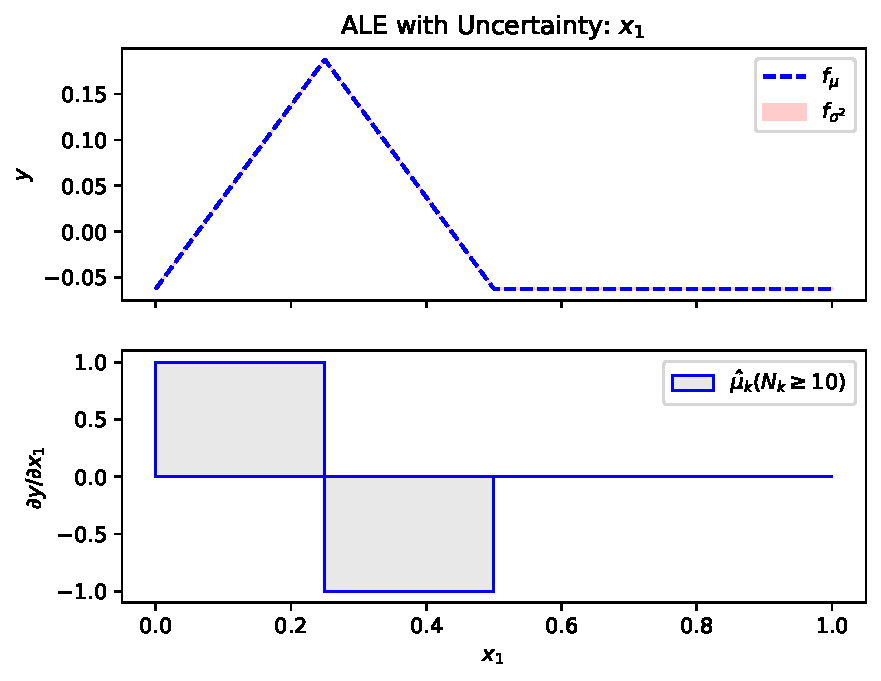
\includegraphics[width=.23\textwidth]{example_1/dale_feat_0.pdf}
  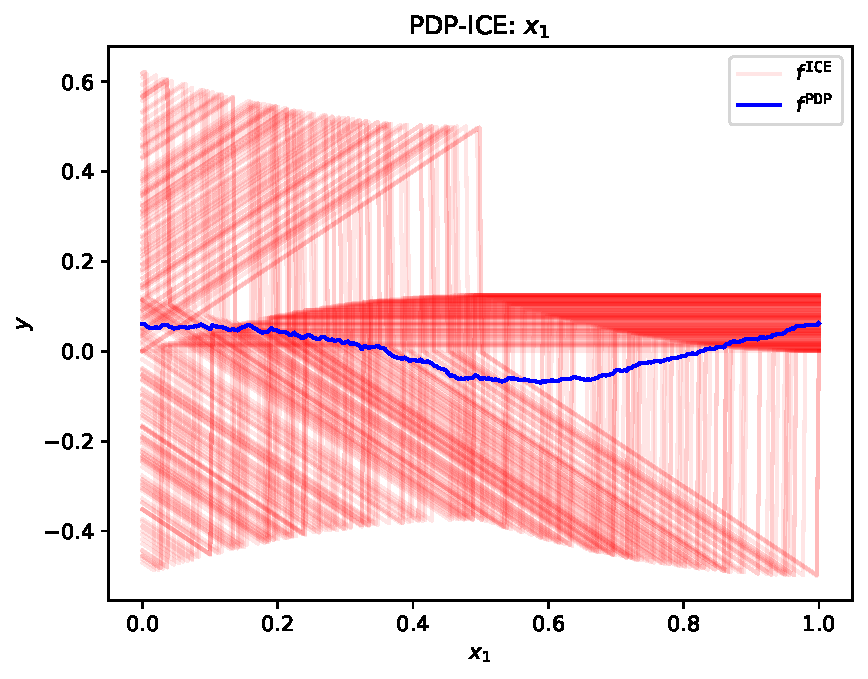
\includegraphics[width=.23\textwidth]{example_1/pdp_ice_feat_0.pdf}
  \caption{No interaction, Equal weights: Feature effect for \(x_1\)
    using UALE (Left) and PDP-ICE (Right).}
  \label{fig:synth-ex-1-case-1}
\end{figure}

\paragraph{(b) No Interaction, Non-Equal Weights.}

Here, \(\alpha=0\) (no interaction), \(a_1 = 2\) and
\(a_2= \frac{1}{2}\) (non-equal weights). The non-equal weights have
implications at both the gradient and the interval of the piece-wise
linear regions, i.e., \(f_\mu^{\mathtt{GT}}(x_1)\) is: \(2x_1\) in
\([0, \frac{1}{5}]\), \(-2x_1\) in \([\frac{1}{5}, \frac{2}{5}]\) and
\(0\) in \([\frac{2}{5}, 1]\). As before, the ground-truth uncertainty
is \(f^{\mathcal{GT}}_{\sigma^2}(x_1) = 0\) because \(x_1\) does not
interact with any other feature. In Figure~\ref{fig:ex-synth-1-2}, we
observe that PDP estimation is opposite to the ground-truth effect,
i.e.~negative in the region \([0, \frac{1}{5})\), positive in
\([\frac{1}{5}, \frac{2}{5})\), and the ICE erroneously implies the
existence of heterogeneous effects. As before, UALE quantifies
correctly the ground truth effect, the zero-uncertainty and partitions
the \(x_1\) domain into wide bins that facilitate the interpretation
and create a zero cummulative bin-error \(\mathcal{E}_{\mathcal{Z}}\)
approximation.

\begin{figure}[h]
  \centering
  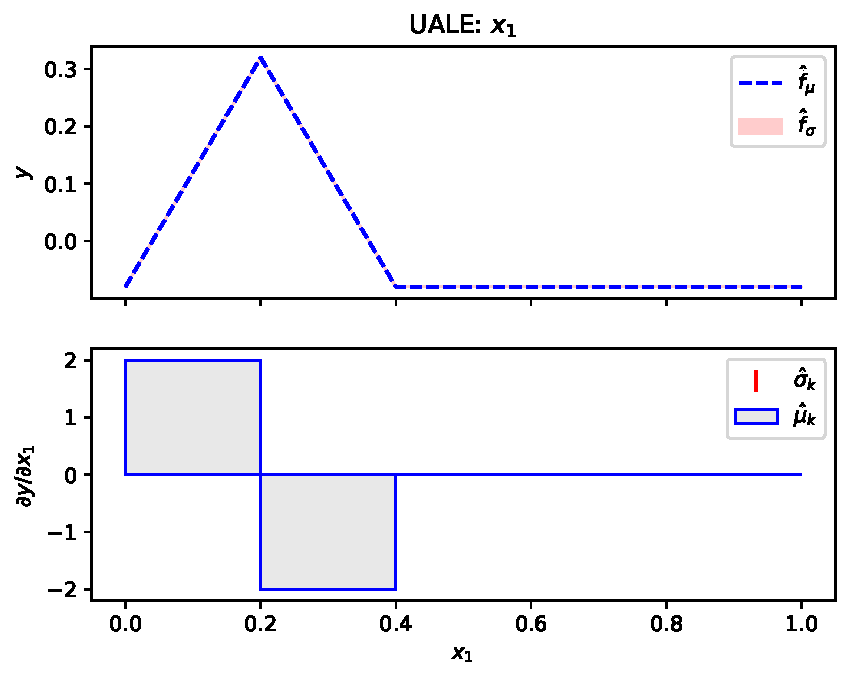
\includegraphics[width=.23\textwidth]{example_2/dale_feat_0.pdf}
  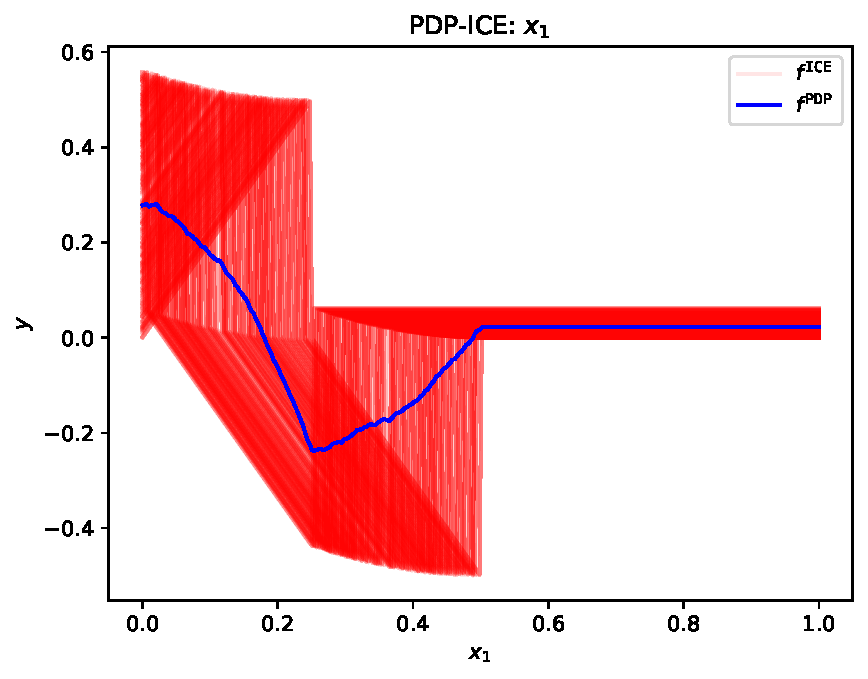
\includegraphics[width=.23\textwidth]{example_2/pdp_ice_feat_0.pdf}
  \caption{No interaction, Different weights: Feature effect for \(x_1\)
    using UALE (Left) and PDP-ICE (Right).}
  \label{fig:ex-synth-1-2}
\end{figure}

\paragraph{(c) With Interaction, Equal weights.}

Here, we activate the interaction term, i.e., \(a=1\), keeping the
weights equal \(a_1=a_2=1\) and \(\sigma_3^2=\frac{1}{4}\). In this
case, it is not straightforward to define the ground-truth effect for
features \(x_1, x_3\), because the interaction term provokes
heterogeneous instance-level effects, i.e., the instance-level effect
of \(x_1\) depend on the unknown value of \(x_3\) and vice-versa. We
observe that UALE's feature effects are quite intuitive. The average
effect of \(x_1\) is the same with the Example (a) with an added
uncertainty, reflecting the uncertainty about the instance-level
effects which is the standard deviation of \(x_3\), i.e.,
\(\sigma_3 = \frac{1}{2}\). The effect of \(x_3\) is only due to the
interaction term, therefore, the instance-level effects
\(\frac{\partial f}{\partial x_3} = x_1 \) follow
\(p(x_1) \sim \mathcal{U}(0,1)\) which has \(\mu_{x_1}=\frac{1}{2}\)
and \(\sigma_{x_1}=\frac{1}{4}\). This is reflected, in UALE's
estimations of Figure~\ref{fig:ex-synth-1-3}.

For \(x_2\), as in Example (a), the effect is
\(f_\mu^{\mathtt{GT}}(x_2)\) is: \(x_2\) in \([0, \frac{1}{4}]\),
\(-x_2\) in \([\frac{1}{4}, \frac{1}{2}]\) and \(0\) in
\([\frac{1}{2}, 1]\)\(x_2\) and it has zero-uncertainty,
\(f_\sigma^{\mathtt{GT}}(x_2) = 0\), since \(x_2\) does not appear in
any interaction term. We confirm that UALE computes it correctly
whereas PDP-ICE fail in both the average effect and the uncertainty.

\begin{figure}[h]
  \centering
  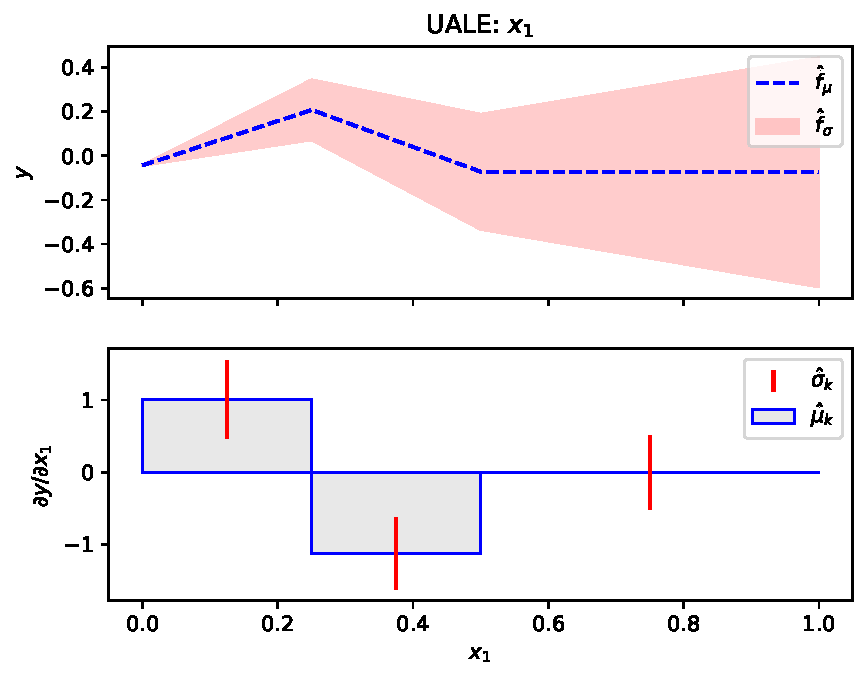
\includegraphics[width=.23\textwidth]{example_3/dale_feat_0.pdf}
  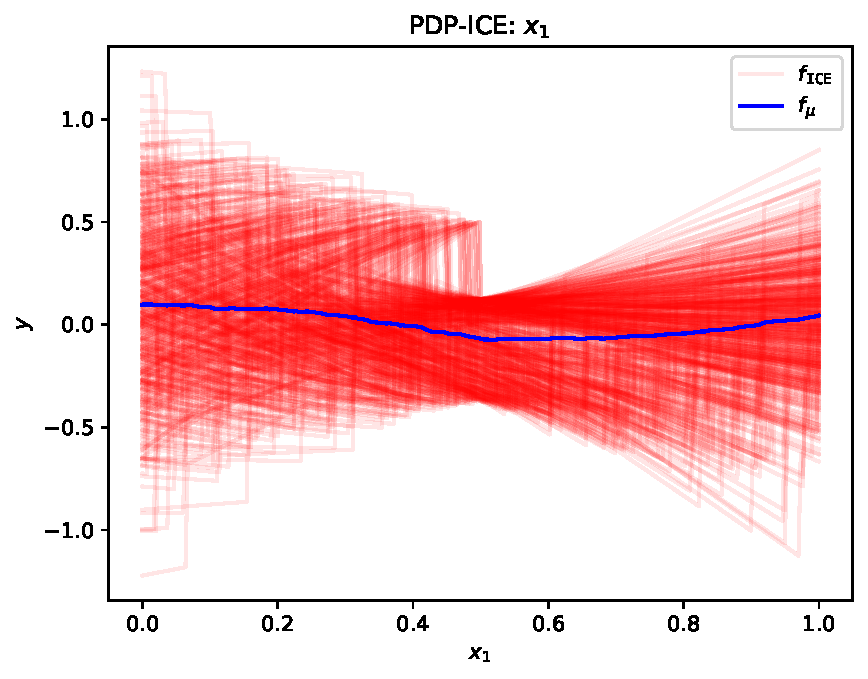
\includegraphics[width=.23\textwidth]{example_3/pdp_ice_feat_0.pdf}\\
  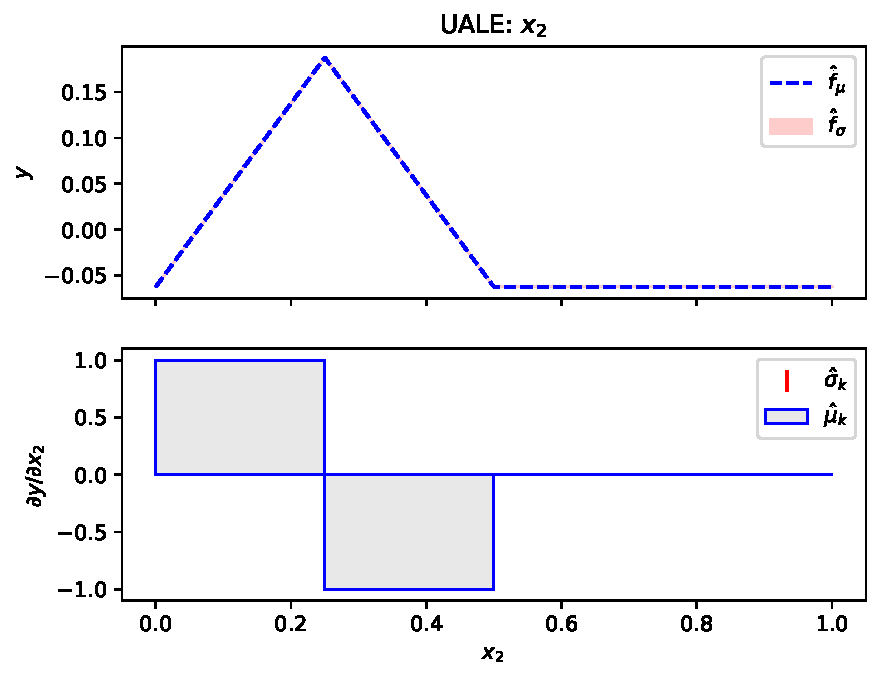
\includegraphics[width=.23\textwidth]{example_3/dale_feat_1.pdf}
  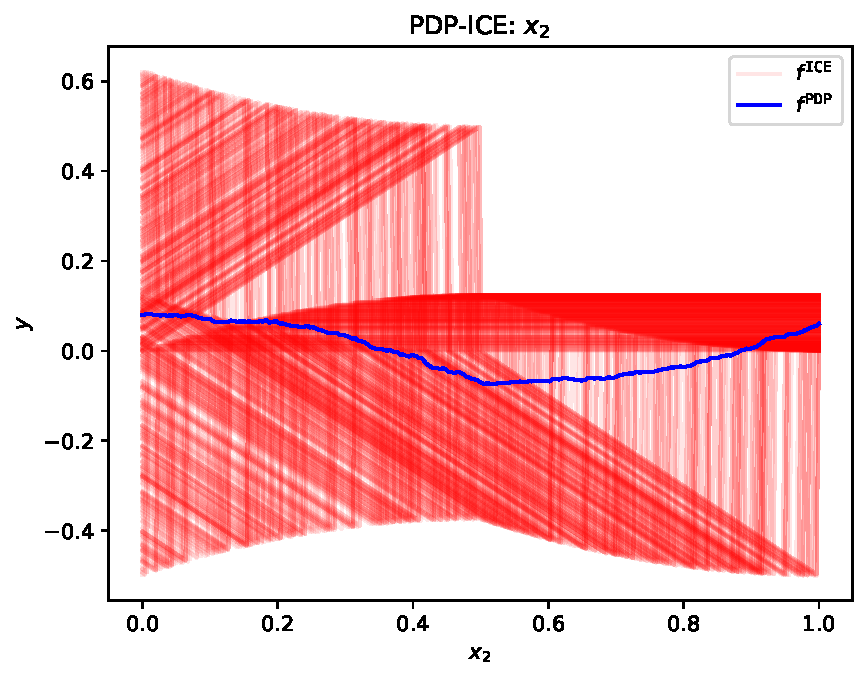
\includegraphics[width=.23\textwidth]{example_3/pdp_ice_feat_1.pdf}\\
  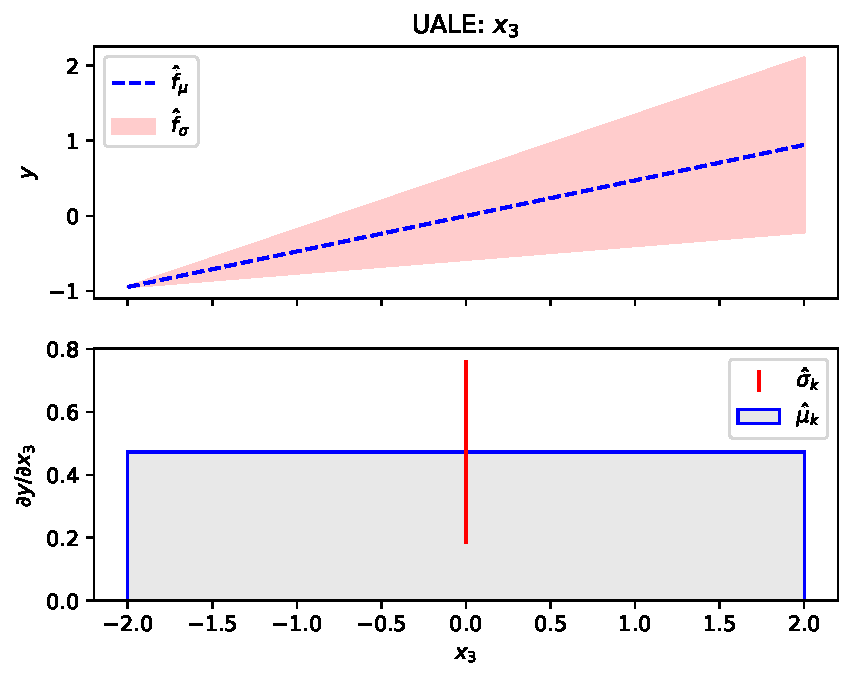
\includegraphics[width=.23\textwidth]{example_3/dale_feat_2.pdf}
  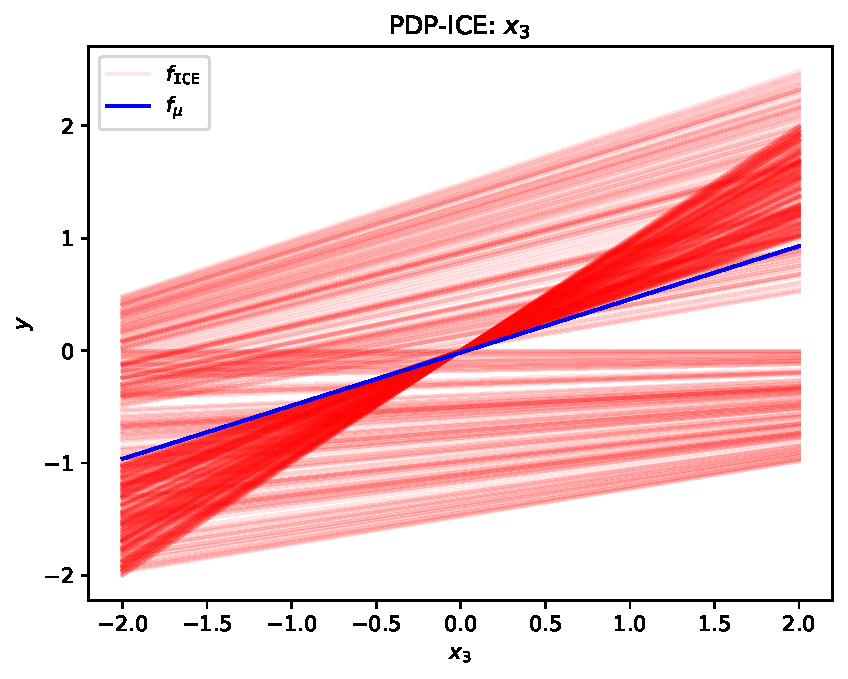
\includegraphics[width=.23\textwidth]{example_3/pdp_ice_feat_2.pdf}\\
  \caption{With interaction, equal weights: From top to bottom,
    feature effect for features \(\{x_1, x_2, x_3\}\) using UALE (left
    column) and PDP-ICE (right column).}
  \label{fig:ex-synth-1-3}
\end{figure}

\paragraph{Discussion.}

The above experiments show that UALE models correctly and estimates
accurately both the average effect and its uncertainty. We also
observed that UALE's variable-size bin-splitting method that we
propose, leads to (a) an accurate approximation of the uncertainty and
(b) favoring wider bins we facilitate the interpretation of both the
average effect and the uncertainty. In contrast, PDP-ICE provides
misleading explanations, due to ignoring correlations between
features. The examples above do not cover the case of an interaction
term between correlated features, for example a term \(x_1x_2\),
because in this case there is an open debate about the ground-truth
effect~\citep{Gromping2020MAEP}.

\subsection{Case 2: Bin-Splitting}
\label{sec:simulation-examples-2}

In this simulation, we illustrate the advantages of automatic
bin-splitting against the fixed-size alternative. For this reason, we
generate a very big dataset applying dense sampling (\(N=10^6\)) and
we treat the estimation with dense fixed-size bins (\(K=10^3\)) as the
ground-truth UALE. Afterwards, we generate fewer samples (\(N=500\))
and we compare the fixed-size estimation (for several \(K\)) against
UALE automatic bin-splitting. In all set-ups, we sample from
\(p(\mathbf{x}) = p(x_2|x_1)p(x_1)\) where
\(x_1 \sim \mathcal{U}(0,1)\) and
\(x_2 \sim \mathcal{N}(x_1, \sigma_2^2=0.5)\). We denote as
\(\mathcal{Z^*} = \{z^*_0, \cdots,
z^*_K\}\) the sequence obtained by automatic
bin-splitting and with \(\mathcal{Z^{\mathtt{K}}}\) the fixed-size
splitting with \(K\) bins. The evaluation metrics we report are the
average number of independent runs \(t = 30\), using each time
\(N=500\) different samples.

\paragraph{Metrics}

Evaluation is perform in terms of the Mean Absolute Error (MAE) of the
estimation of \(\mu\) and \(\sigma\) accross bins, i.e.,

% The evaluation is done with regard to two metrics counting the mean
% error per bin, where the bin error is definde as the absolute
% difference of the approximation from the ground-truth. The first
% metric, Eq.~\eqref{eq:eval_met_1}, counts the mean bin error wrt
% average effect and the second, Eq.~\eqref{eq:eval_met_2} the mean bin
% error wrt uncertainty:

\begin{equation}
  \label{eq:eval_met_1}
  \mathcal{L}^{\mu} = \frac{1}{|\mathcal{Z}|} \sum_{k \in
  \mathcal{Z}} | \mu(z_{k-1}, z_k) - \hat{\mu}(z_{k-1}, z_k) |
\end{equation}


\begin{equation}
  \label{eq:eval_met_2}
  \mathcal{L}^{\sigma} = \frac{1}{|\mathcal{Z}|} \sum_{k \in
    \mathcal{Z}} | \sigma(z_{k-1}, z_k) - \hat{\sigma}(z_{k-1}, z_k) |
\end{equation}

The ground truth UALE is the average of the dense fixed-size bins that
are within in the interval \([z_{k-1}, z_k]\). For better
interpretation of \(\mathcal{L}^{\sigma}\), we also provide the mean
error term
\(\mathcal{L}^{\rho} = \frac{1}{|\mathcal{Z}|} \sum_{k \in
  \mathcal{Z}} \mathcal{E}(z_{k-1}, z_k) \).

\paragraph{Piecewise-Linear Function.}

In this set-up, \(f(\mathbf{x}) = a_1x_1 + x_1x_2\) is a
piecewise-linear function with \(5\) different-width regions, i.e.,
\(a_1\) equals to \(\{2, -2, 5, -10, 0.5\}\) in the intervals defined
by the sequence \(\{0, 0.2, 0.4, 0.45, 0.5, 1\}\).

As we observe in the top left of Figure~\ref{fig:ex-synth-2-1}, UALE's
bin-splitting separates the fine-grained bins, e.g.~regions
\([0.4, 0.45]\), \([0.45, 0.5]\), and unites (most) constant-effect
regions into a single bin, e.g.~region \([0.5, 1]\). This explains the
fact that UALE achieves lower MAE \(\mathcal{L}^{\mu}\),
\(\mathcal{L}^{\sigma}\) compared to fixed-size bins for all \(K\).


% We observe that in
% this case all intervals are multiples of \(0.05\). As we observe, in
% Figure~\ref{fig:ex-synth-2-1}, UALE's approximation is better than all
% fixed-size alternatives (for all \(K\)), in both mean effect
% \(\mathcal{L}^{\mu}\) and uncertainty \(\mathcal{L}^{\sigma}\). For
% understanding the importance of variable-size splitting, we analyze
% the fixed-bin error. In the top-right of
% Figure~\ref{fig:ex-synth-2-1}, we observe a positive trend between
% \(\mathcal{L}^{\mu}\) and \(K\), because as \(K\) becomes larger fewer
% points contribute to the bin estimations, leading to a worse
% approximation. The interpretation of \(\mathcal{L}^{\sigma}\) is more
% complex. For \(K\) that are multiples of \(20\), i.e.
% \(K=\{20, 40, 60, 80, 100\}\), the mean error term
% \(\mathcal{L}^{\rho}\) is low as we see in the bottom-right of
% Figure~\ref{fig:ex-synth-2-2}. In these cases, we also observe in the
% bottom-left figure, that \(L\) is increasing with \(K\) due to fewer
% points in each bin. For all other values of \(K\), the \(L\) is mainly
% affected by the mean error term \(\mathcal{E}\).


\begin{figure}[h]
  \centering
  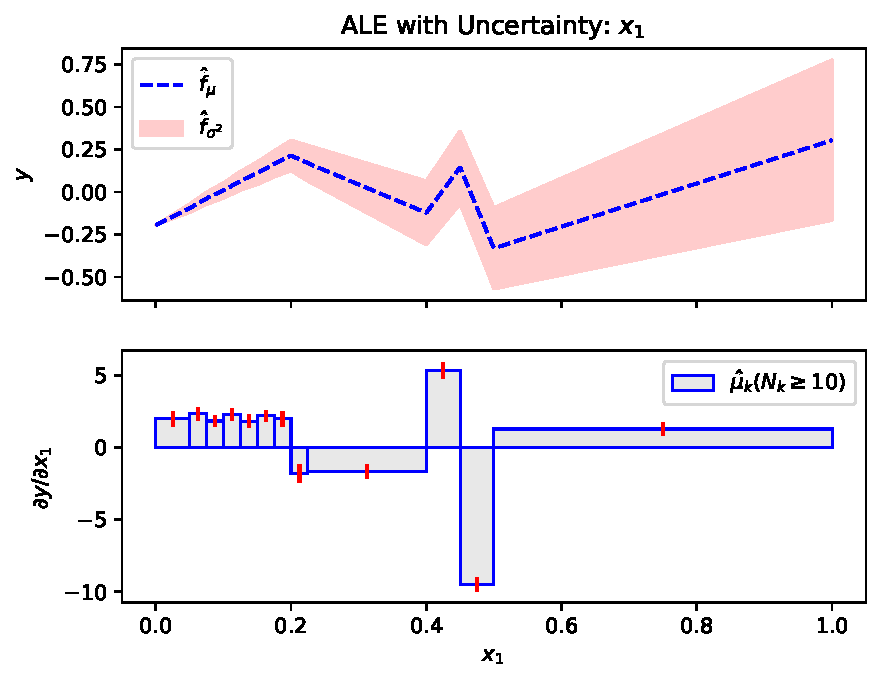
\includegraphics[width=.23\textwidth]{example_bin_splitting_1/fig_1.pdf}
  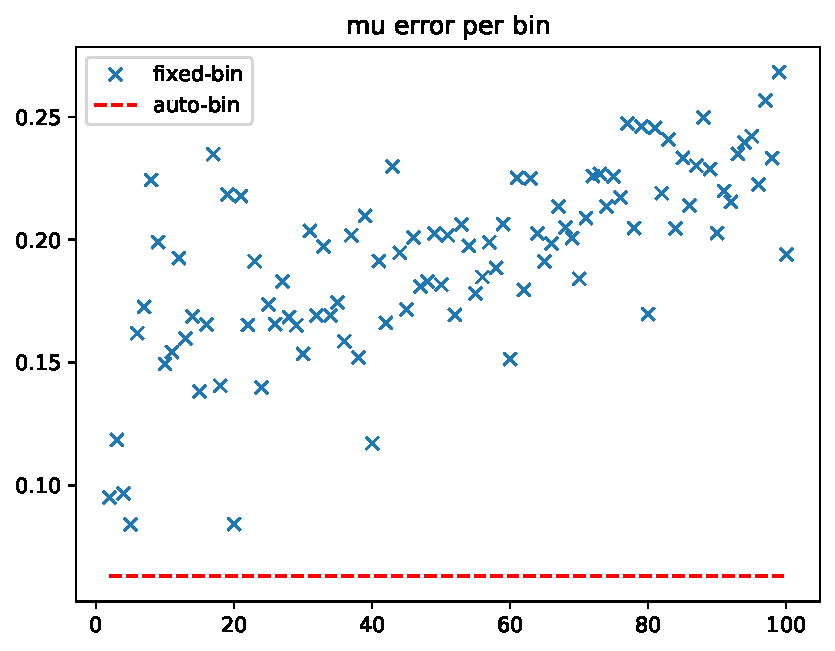
\includegraphics[width=.23\textwidth]{example_bin_splitting_1/fig_2.pdf}\\
  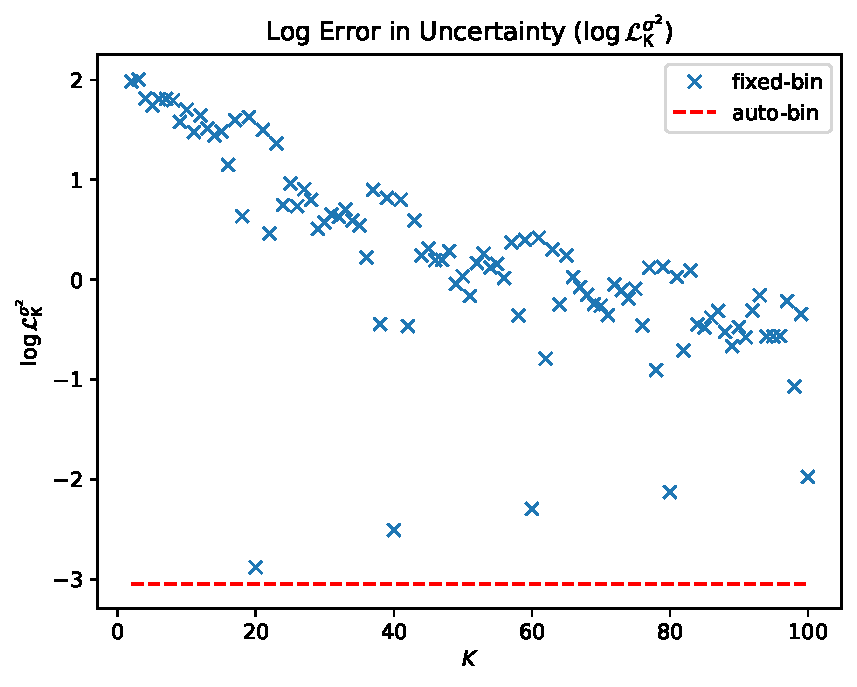
\includegraphics[width=.23\textwidth]{example_bin_splitting_1/fig_3.pdf}
  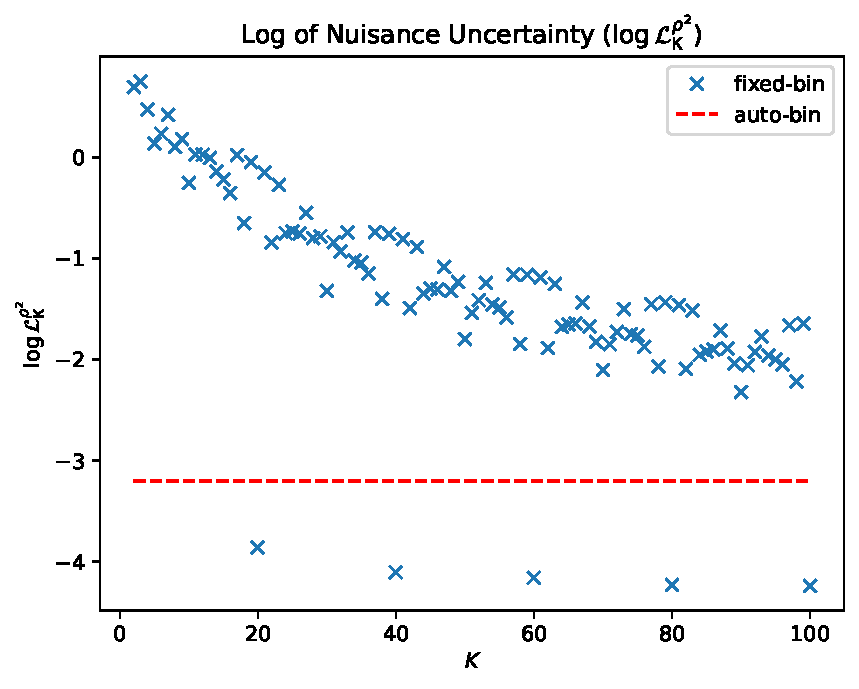
\includegraphics[width=.23\textwidth]{example_bin_splitting_1/fig_4.pdf}
  \caption{Figure 1}
  \label{fig:ex-synth-2-1}
\end{figure}


\paragraph{Non-Linear Function.}

In this set-up, \(f(\mathbf{x}) = 4x_1^2 + x_2^2 + x_1x_2\), so the
effect is non-linear in \(0 \leq x_1 \leq 1\). Due to this non
linearity, wide bins increase \(\mathcal{L}^{\rho}\) making the
uncertainty approximation biased. On the other hand, narrow bins lead
to worse approximation due to the limited number of
samples. Interestingly, in Figure~\ref{fig:ex-synth-2-2}, we observe
that UALE's bin splitting manages to compromise these conflicting
objectives.

\begin{figure}[h]
  \centering
  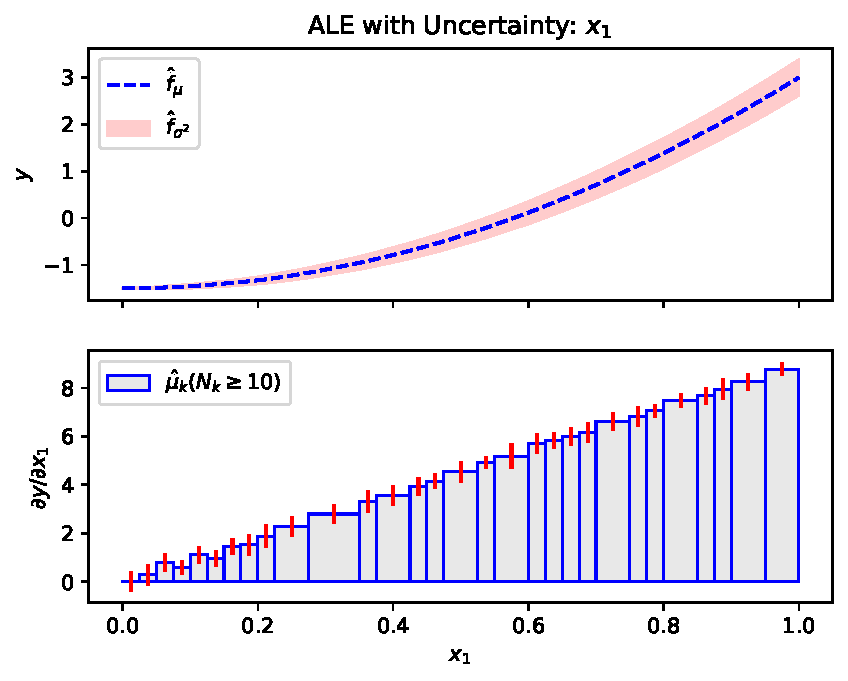
\includegraphics[width=.23\textwidth]{example_bin_splitting_2/fig_1.pdf}
  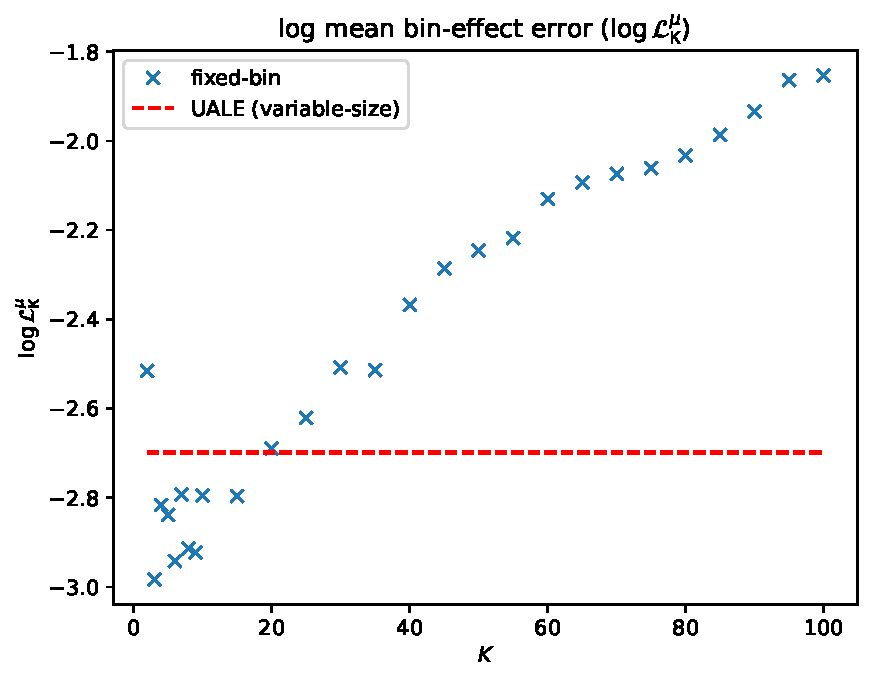
\includegraphics[width=.23\textwidth]{example_bin_splitting_2/fig_2.pdf}\\
  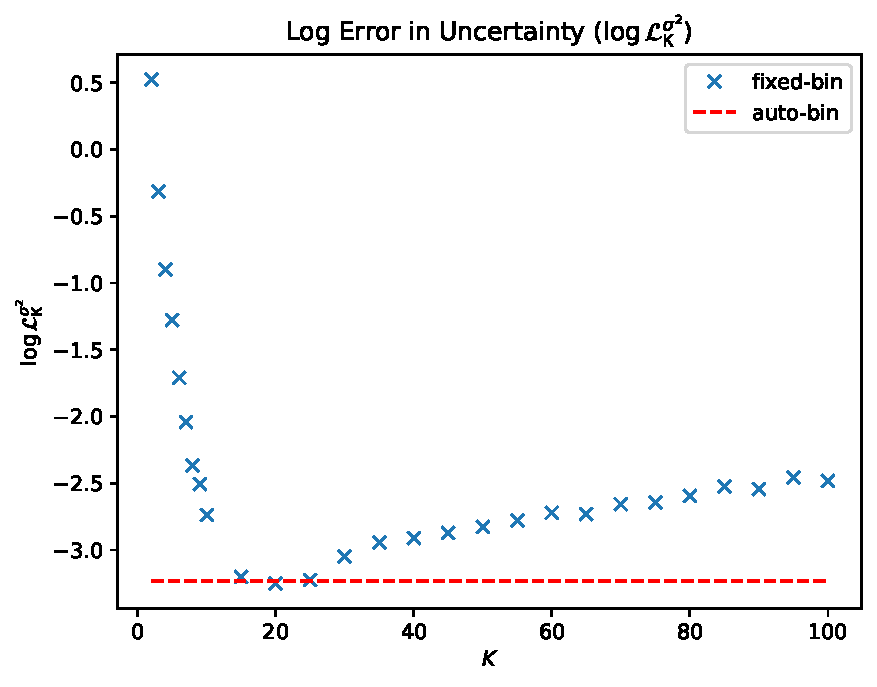
\includegraphics[width=.23\textwidth]{example_bin_splitting_2/fig_3.pdf}
  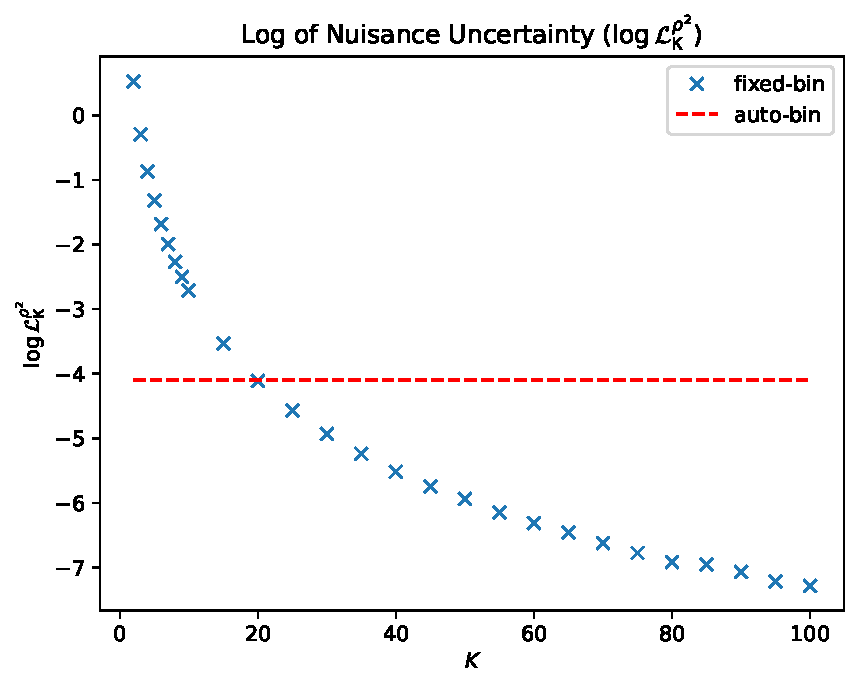
\includegraphics[width=.23\textwidth]{example_bin_splitting_2/fig_4.pdf}
  \caption{Figure 1}
  \label{fig:ex-synth-2-2}
\end{figure}

\section{REAL-WORLD EXAMPLE}

Here, we aim at demonstrating the usefuleness of uncertainty
quantification and the advantages of UALE's approximation, on the
real-world California Housing dataset~\citep{pace1997sparse}.

\paragraph{ML setup}

The California Housing is a largely-studied dataset with approximately
\(20000\) training instances, making it appropriate for robust
approximation with large \(K\). The dataset contains \(D=8\) numerical
features with characteristics about the building blocks of California,
e.g. latitude, longitude, population of the block or median age of
houses in the block. The target variable is the median value of the
houses inside the block in dollars that ranges between
\([15, 500] \cdot 10^3\), with a mean value of
\(\mu_Y \approx 201 \cdot 10^3 \) and a standard deviation of
\(\sigma_Y \approx 110 \cdot 10^3\).

We exclude instances with missing and outlier values. As outlier we
define the feature values which ar over three standard deviations away
from the mean feature value. We also normalize all features to
zero-mean and unit standard deviation. We split the dataset into
\(N_{tr} = 15639\) training and \(N_{test} = 3910\) test examples
(80/20 split) and we fit a Neural Network with 3 hidden layers of 256,
128 and 36 units respectively. After 15 epochs using the Adam
optimizer with learning rate \(\eta = 0.02\), the model achieves a MAE
of \(37 \cdot 10^3\) dollars.

Below, we illustrate the feature effect for three features: latitude
\(x_2\), population \(x_6\) and median income \(x_8\). The particular
features cover the main FE cases, e.g.~positive/negative trend and
linear/non-linear curve, and are therefore appropriate for
illustration purposes. Results for all features, along with in-depth
information about the preprocessing, training and evaluation parts are
provided in the Appendix.

\paragraph{Uncertainty Quantification}

In real-world datasets, it is infeasible to obtain the ground truth FE
for evaluation. We observe in Figure \ref{fig:ex-real-1} that in broad
terms UALE and PDP-ICE plots aggree on the average effect and the
uncertainty. It is interesting to note that UALE has selected bins of
varying size as the optimal partiotioning. This demonstrates an
important advantage of UALE; through the bin splitting process we can
identify wide intervals of the feature domain with similar level of
uncertainty.

% We selected the particular experiment, because, in
% broad terms, UALE and PDP-ICE plots aggree in the estimation of the
% average effect and uncertainty. Therefore, we can focus on juding the
% quality of the information provided by the two methods.

% In Figure\ref{fig:ex-real-1}, we observe, from top to bottom, the
% effects for the latitude, population and the median income. The effect
% of UALE and PDP-ICE are similar for the population and the median
% income. The population has a negative impact that progressively
% decreases: from 400 to 1500 people the house value decreases with a
% rate of \(-150 (\pm 140)\) dollars per added person, a rate that
% decreases from \(-80 (\pm 80)\) to \(-60 (\pm 60)\) dollars per added
% person as we move from 1500 to 2800 people. The level of uncertainty
% indicates significant variance in absolute value of the rate, but in
% the grant majority of instances the rate is negative. With the same
% inspection, we observe that the median annual income has a positive
% impact on the value (all numbers are thousands of dollars):
% \(20\pm 15\) per \(10\) of added median income for incomes in
% \([8, 15]\), \(32 \pm 20\) per \(10\) added income in \([15, 60]\) and
% \(40 \pm 15\) per \(10\) added income in \([60, 70]\). The uncertainty
% indicates that there are less heterogeneous effects about the median
% income compared to the number of people. In both cases, we can end-up
% to the same conclusion by inspecting the PDP-ICE plots. For the
% latitude, there is a small difference in the explanations for the
% region \([32, 35]\), where UALE estimates a less negative slope with
% less uncertainty than PDP, while the explanations are similar for the
% range \([35,39]\), where both methods reveal an increase in the
% uncertainty around the feature value \(37.5\).

% In general, we observe that UALE complements ALE in the quantification
% of the heterogeneous effects, similarly to as ICE complements PDP. The
% automatic extraction of constant-effect and constant-uncertainty
% regions provided by UALE is helpful for an easier interpretation.

% On
% the other hand, ICE plots sometimes are more descritive due to
% illustrating the type of heterogeneity, whereas UALE quantifies only the
% level (not the type) of heterogeneity.

\begin{figure}[h]
  \centering
  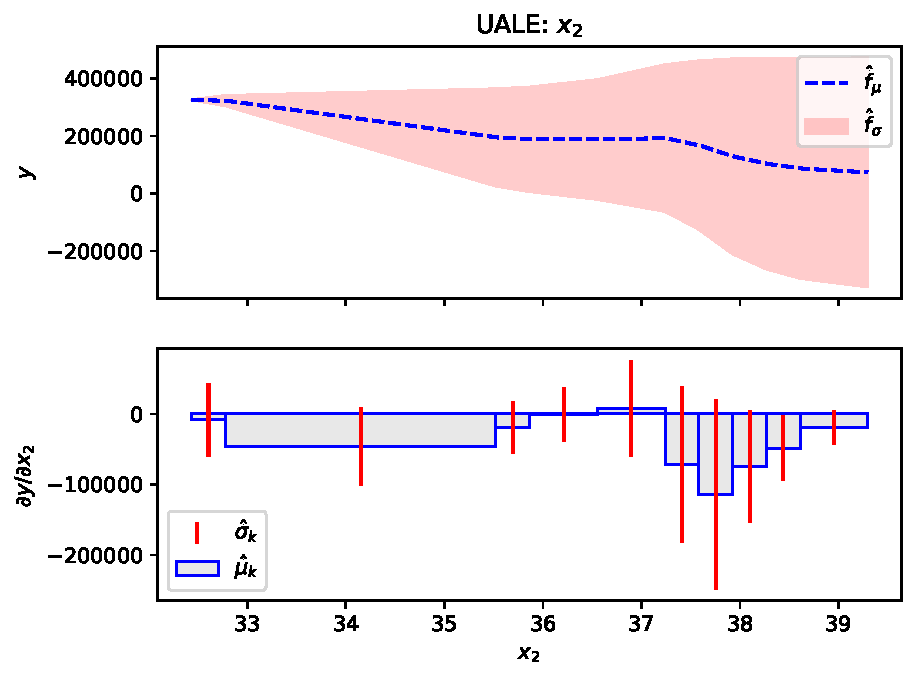
\includegraphics[width=.23\textwidth]{real_dataset_3/feature_1_ale_auto.pdf}
  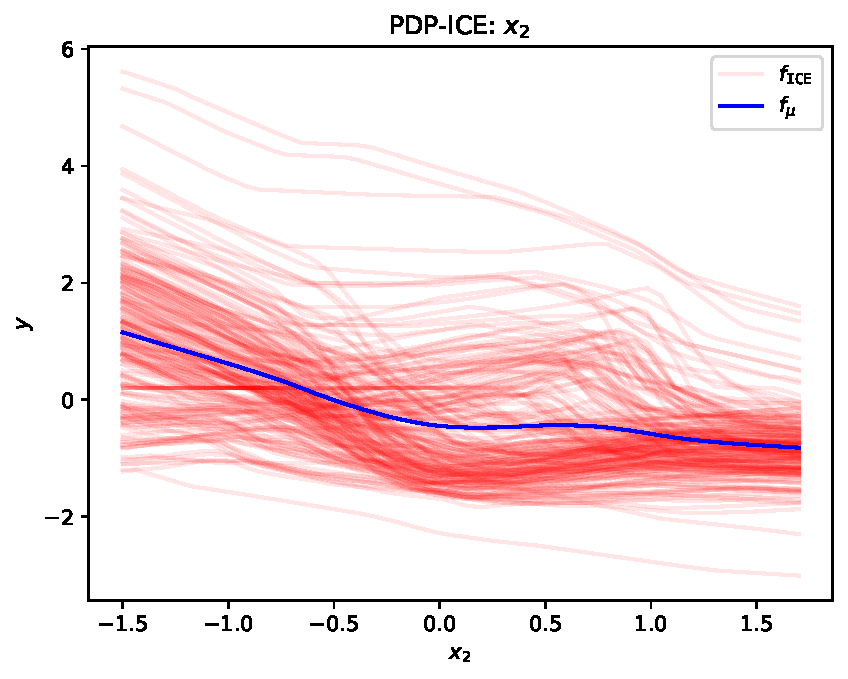
\includegraphics[width=.23\textwidth]{real_dataset_3/feature_1_pdp_ice.pdf}\\
  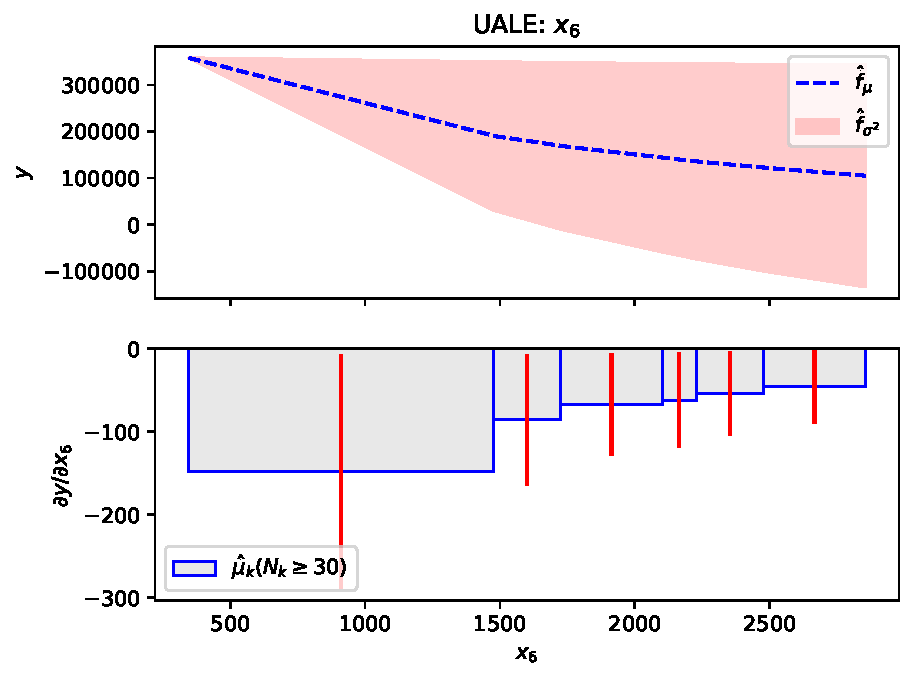
\includegraphics[width=.23\textwidth]{real_dataset_3/feature_5_ale_auto.pdf}
  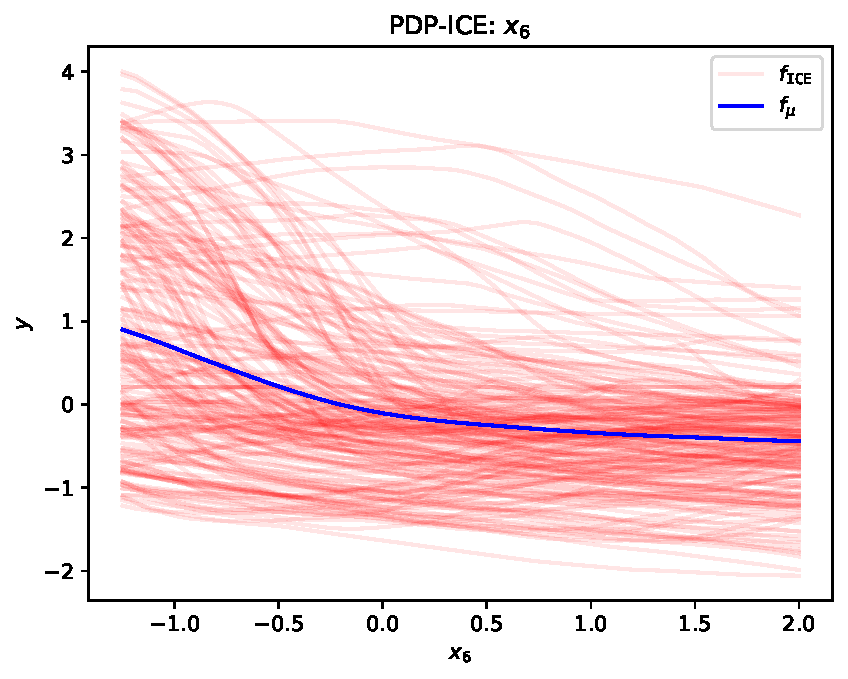
\includegraphics[width=.23\textwidth]{real_dataset_3/feature_5_pdp_ice.pdf}\\
  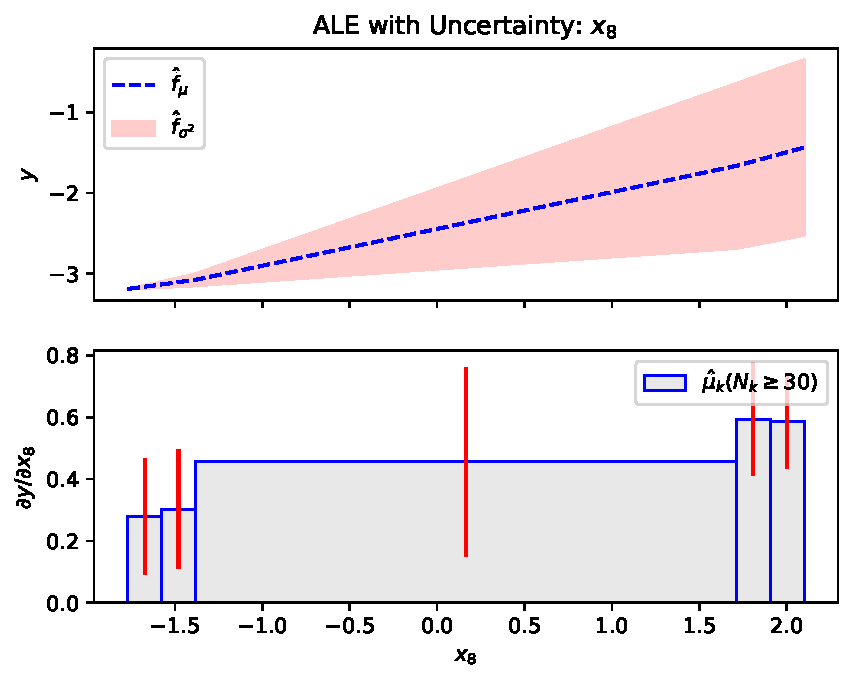
\includegraphics[width=.23\textwidth]{real_dataset_3/feature_7_ale_auto.pdf}
  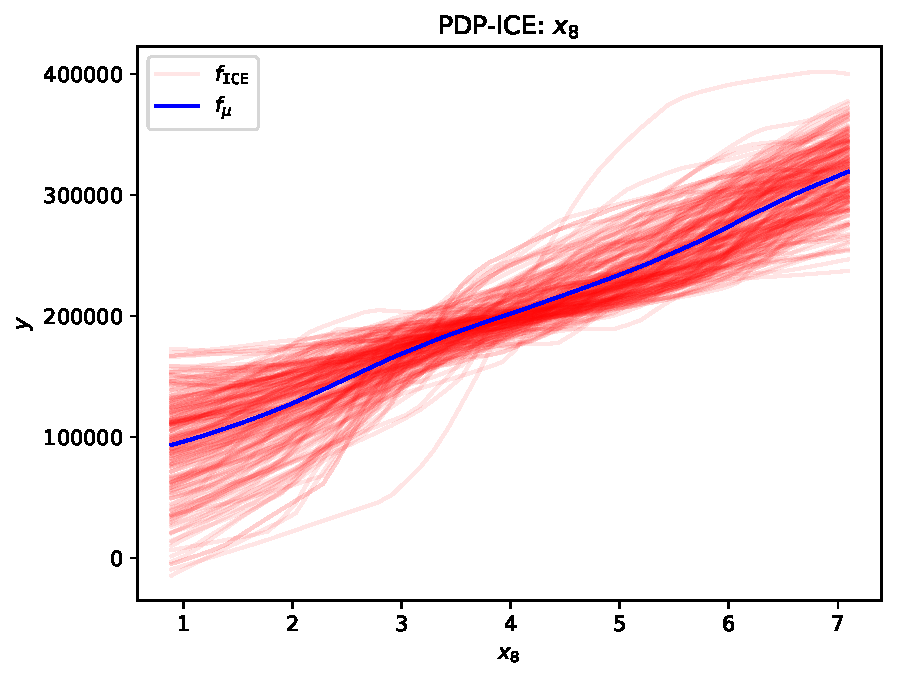
\includegraphics[width=.23\textwidth]{real_dataset_3/feature_7_pdp_ice.pdf}\\
  \caption{Figure 1}
  \label{fig:ex-real-1}
\end{figure}

\paragraph{Bin Splitting}

We evaluate the robustness of UALE approximation. Following the
evaluation framework of Section~\ref{sec:simulation-examples-2}, we
treat as ground-truth the effects computed on the full training-set
\(N=20000\) with dense fixed-size bin-splitting (\(K=80\)). Given the
big number of samples, we make the hypothesis that the approximation
with dense binning is close to the ground truth. Afterwards, we
randomly select fewer samples, \(N=1000\), and we compare UALE
approximation with all possible fixed-size approximation. We repeat
this process \(t=30\) times. In Figure~\ref{fig:ex-real-2}, we
illustrate the mean values of
\(\mathcal{L}^{\mu}, \mathcal{L}^{\sigma}\) across the 30
repetitions. We observe that UALE achieves (near) optimal
approximation in all cases. \todo{add explanation for near-constant
  feature effect vs the first case that the plot }

\begin{figure}[h]
  \centering
  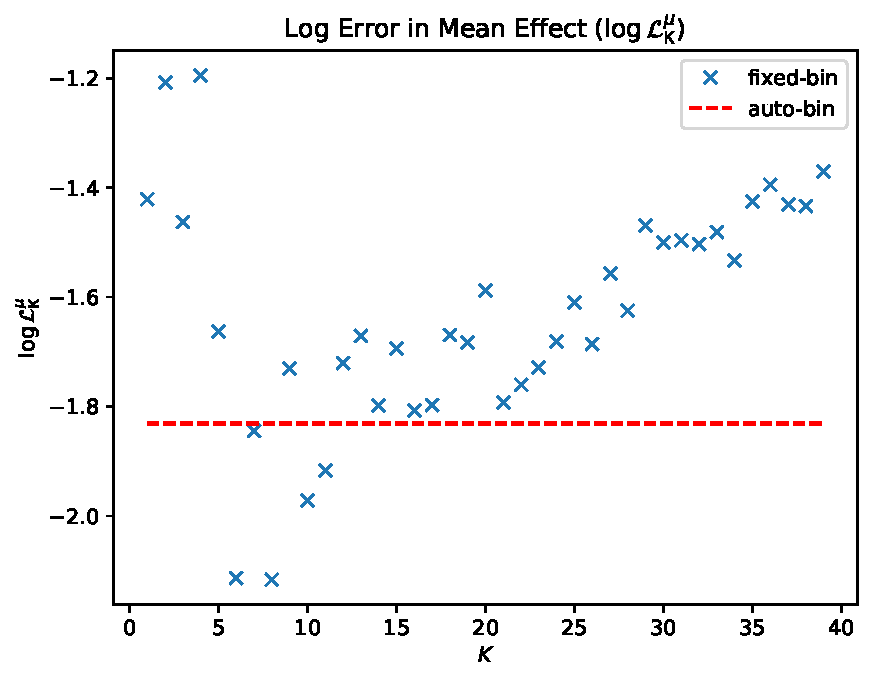
\includegraphics[width=.23\textwidth]{real_dataset_3/compare_mu_err_feature_1.pdf}
  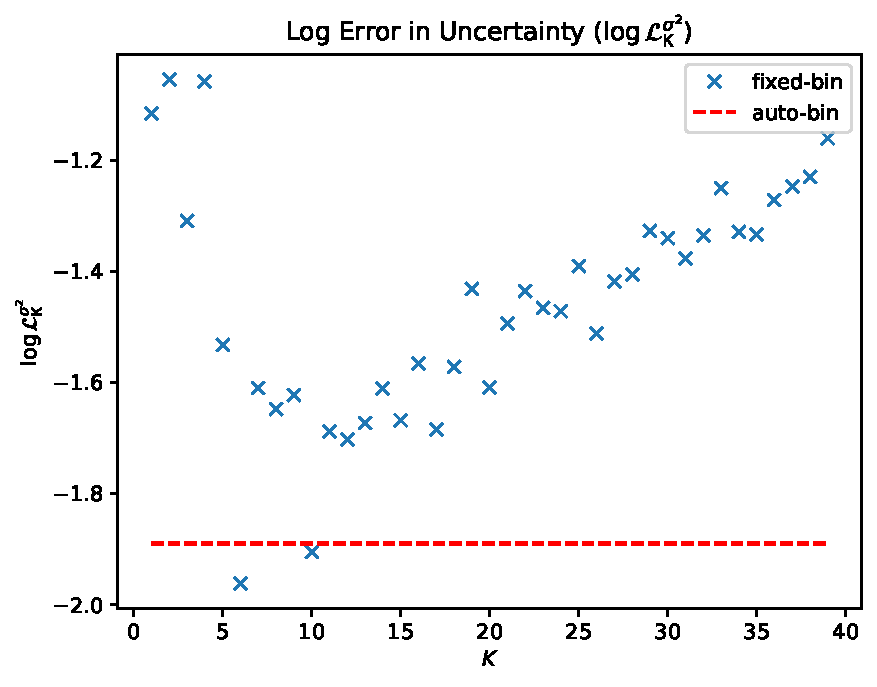
\includegraphics[width=.23\textwidth]{real_dataset_3/compare_var_err_feature_1.pdf}\\
  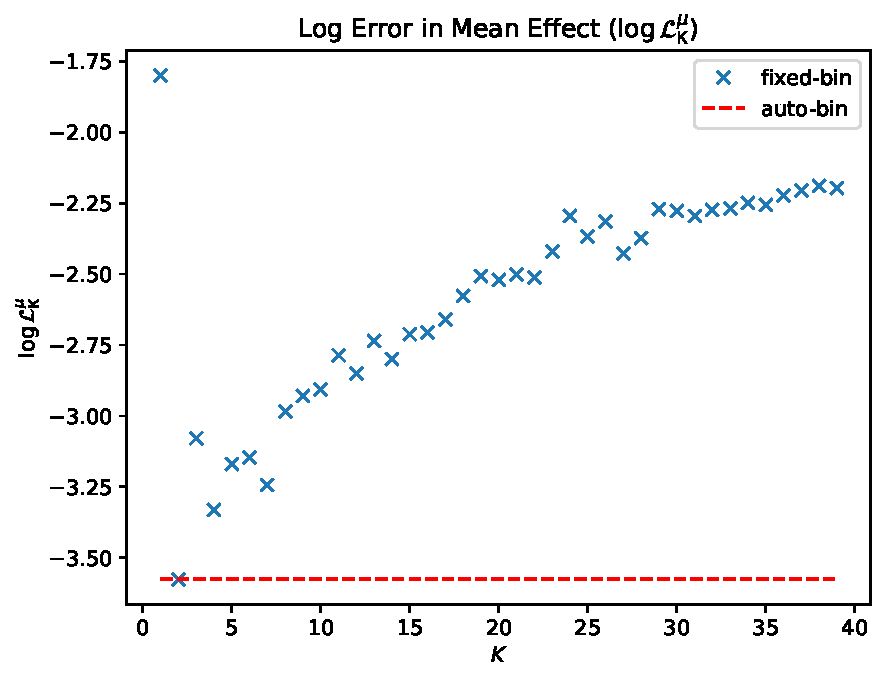
\includegraphics[width=.23\textwidth]{real_dataset_3/compare_mu_err_feature_5.pdf}
  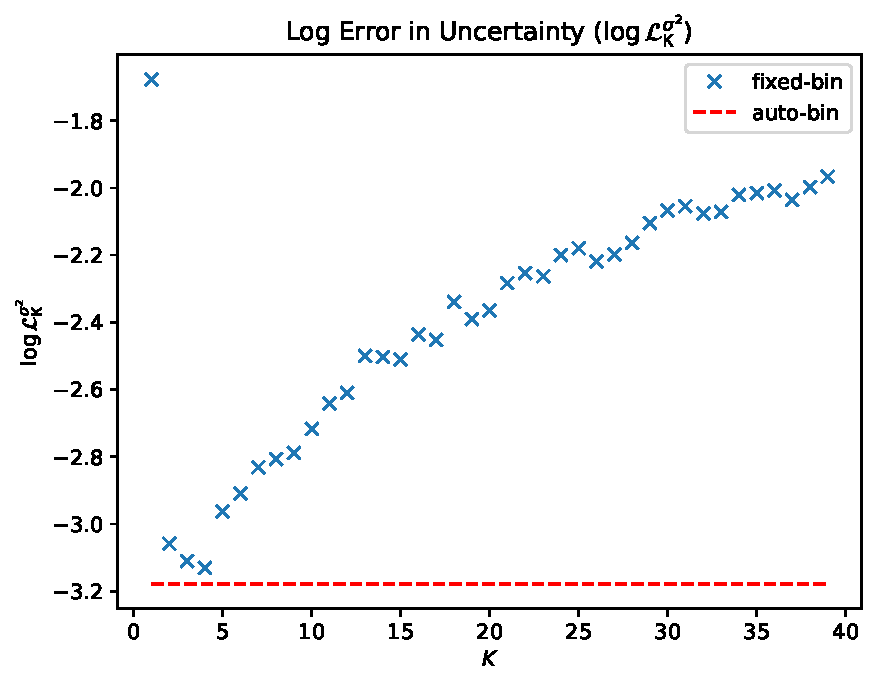
\includegraphics[width=.23\textwidth]{real_dataset_3/compare_var_err_feature_5.pdf}\\
  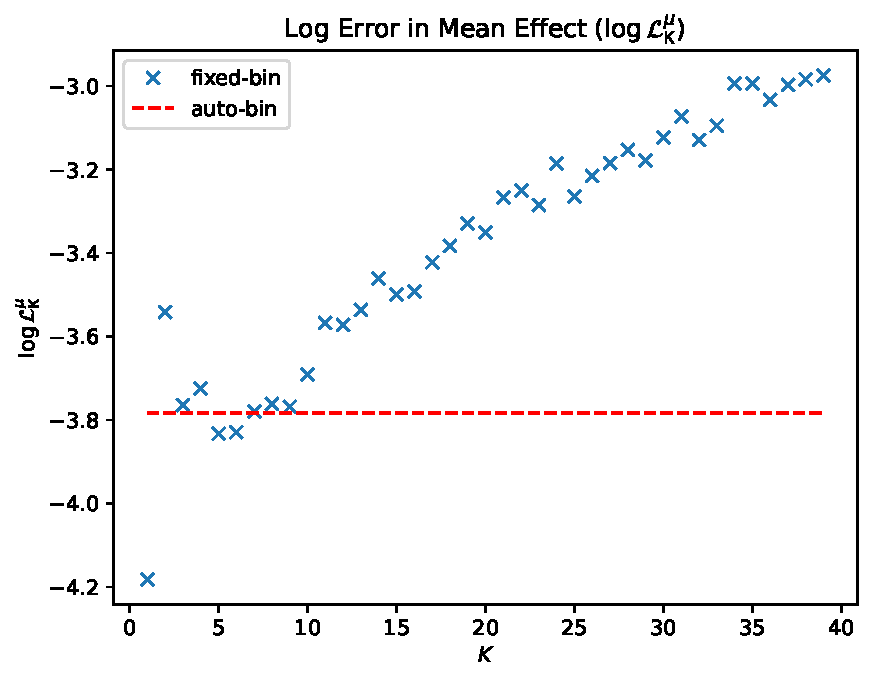
\includegraphics[width=.23\textwidth]{real_dataset_3/compare_mu_err_feature_7.pdf}
  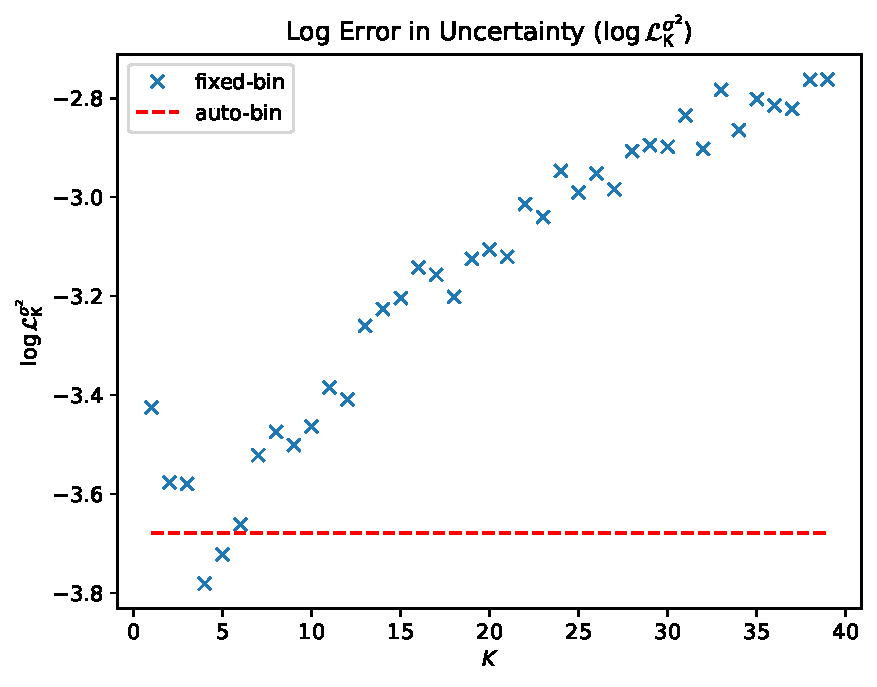
\includegraphics[width=.23\textwidth]{real_dataset_3/compare_var_err_feature_7.pdf}\\
  \caption{Figure 1}
  \label{fig:ex-real-2}
\end{figure}

\section{DISCUSSION}

\todo{Add Conclusion, limitations, and future work}

\subsubsection*{Acknowledgments}
All acknowledgments go at the end of the paper, including thanks to reviewers who gave useful comments, to colleagues who contributed to the ideas, and to funding agencies and corporate sponsors that provided financial support. 
To preserve the anonymity, please include acknowledgments \emph{only} in the camera-ready papers.

\bibliography{biblio}

\appendix

\section{List with Symbols}
\label{sec:list-with-symbols}

\section{Show that is unbiased estimator}
\label{sec:proof-1}

\section{Proof of Theorem~\ref{sec:theorem-1}}
\label{sec:proof-of-3-1}

\section{Proof of Corollary~\ref{sec:coroll-1}}
\label{sec:proof-of-coroll}

\section{Dynamic Programming}
\label{sec:dynamic-programming}

\todo{Review all the description}
For achieving a computationally-grounded solution we set a threshold
\(K_{max}\) on the maximum number of bins which also discretizes the
solution space. The width of the bin can take discrete values that are
multiple of the minimum step
\(u = \frac{x_{s, max} - x_{s, min}}{K_{max}}\). For defining the
solution, we use two indexes. The index
\(i \in \{0, \ldots, K_{max}\}\) denotes the point \((z_i)\) and the
index \(j \in \{0, \ldots, K_{max}\} \) denotes the position of the
\(j\)-th multiple of the minimum step, i.e., 
\(x_j = x_{s,min} + j \cdot u\). The recursive cost function
\(T(i,j)\) is the cost of setting \(z_i=x_j\):
\begin{equation}
  \label{eq:recursive_cost}
  \mathcal{T}(i,j) = \mathrm{min}_{l \in \{0, \ldots, K_{max}\}} \left [ \mathcal{T}(i-1, l) + \mathcal{B}(x_l, x_j) \right ]
\end{equation}
%
where \(\mathcal{T}(0,j)\) equals zero if \(j=0\) and \(\infty\) in
any other case. \(\mathcal{B}(x_l, x_j)\) denotes the cost of creating a bin
with limits \([x_l, x_j)]\):

\begin{equation}
  \label{eq:cost_step}
  \mathcal{B}(x_l, x_j) = \begin{cases}
                            \infty, & \text{if $x_j > x_l$ or \(|\mathcal{S}_{(x_j, x_l)}| < N\)}\\
                            0, & \text{if $x_j = x_l$}\\
                            \hat{\sigma}^2(x_j, x_l), &\text{if $x_j \leq x_l$}
  \end{cases}
\end{equation}

The optimal solution is given by solving
\(\mathcal{L} = \mathcal{T}(K_{max}, K_{max})\) and keeping track of the sequence of
steps. 

\noindent

\begin{itemize}
\item Discuss more aspects (e.g. Computational complexity)
\end{itemize}


\end{document}
